\documentclass[twoside]{book}

% Packages required by doxygen
\usepackage{fixltx2e}
\usepackage{calc}
\usepackage{doxygen}
\usepackage[export]{adjustbox} % also loads graphicx
\usepackage{graphicx}
\usepackage[utf8]{inputenc}
\usepackage{makeidx}
\usepackage{multicol}
\usepackage{multirow}
\PassOptionsToPackage{warn}{textcomp}
\usepackage{textcomp}
\usepackage[nointegrals]{wasysym}
\usepackage[table]{xcolor}

% NLS support packages
\usepackage[T2A]{fontenc}
\usepackage[russian]{babel}

% Font selection
\usepackage[T1]{fontenc}
\usepackage[scaled=.90]{helvet}
\usepackage{courier}
\usepackage{amssymb}
\usepackage{sectsty}
\renewcommand{\familydefault}{\sfdefault}
\allsectionsfont{%
  \fontseries{bc}\selectfont%
  \color{darkgray}%
}
\renewcommand{\DoxyLabelFont}{%
  \fontseries{bc}\selectfont%
  \color{darkgray}%
}
\newcommand{\+}{\discretionary{\mbox{\scriptsize$\hookleftarrow$}}{}{}}

% Page & text layout
\usepackage{geometry}
\geometry{%
  a4paper,%
  top=2.5cm,%
  bottom=2.5cm,%
  left=2.5cm,%
  right=2.5cm%
}
\tolerance=750
\hfuzz=15pt
\hbadness=750
\setlength{\emergencystretch}{15pt}
\setlength{\parindent}{0cm}
\setlength{\parskip}{3ex plus 2ex minus 2ex}
\makeatletter
\renewcommand{\paragraph}{%
  \@startsection{paragraph}{4}{0ex}{-1.0ex}{1.0ex}{%
    \normalfont\normalsize\bfseries\SS@parafont%
  }%
}
\renewcommand{\subparagraph}{%
  \@startsection{subparagraph}{5}{0ex}{-1.0ex}{1.0ex}{%
    \normalfont\normalsize\bfseries\SS@subparafont%
  }%
}
\makeatother

% Headers & footers
\usepackage{fancyhdr}
\pagestyle{fancyplain}
\fancyhead[LE]{\fancyplain{}{\bfseries\thepage}}
\fancyhead[CE]{\fancyplain{}{}}
\fancyhead[RE]{\fancyplain{}{\bfseries\leftmark}}
\fancyhead[LO]{\fancyplain{}{\bfseries\rightmark}}
\fancyhead[CO]{\fancyplain{}{}}
\fancyhead[RO]{\fancyplain{}{\bfseries\thepage}}
\fancyfoot[LE]{\fancyplain{}{}}
\fancyfoot[CE]{\fancyplain{}{}}
\fancyfoot[RE]{\fancyplain{}{\bfseries\scriptsize Создано системой Doxygen }}
\fancyfoot[LO]{\fancyplain{}{\bfseries\scriptsize Создано системой Doxygen }}
\fancyfoot[CO]{\fancyplain{}{}}
\fancyfoot[RO]{\fancyplain{}{}}
\renewcommand{\footrulewidth}{0.4pt}
\renewcommand{\chaptermark}[1]{%
  \markboth{#1}{}%
}
\renewcommand{\sectionmark}[1]{%
  \markright{\thesection\ #1}%
}

% Indices & bibliography
\usepackage{natbib}
\usepackage[titles]{tocloft}
\setcounter{tocdepth}{3}
\setcounter{secnumdepth}{5}
\makeindex

% Hyperlinks (required, but should be loaded last)
\usepackage{ifpdf}
\ifpdf
  \usepackage[pdftex,pagebackref=true]{hyperref}
\else
  \usepackage[ps2pdf,pagebackref=true]{hyperref}
\fi
\hypersetup{%
  colorlinks=true,%
  linkcolor=blue,%
  citecolor=blue,%
  unicode%
}

% Custom commands
\newcommand{\clearemptydoublepage}{%
  \newpage{\pagestyle{empty}\cleardoublepage}%
}

\usepackage{caption}
\captionsetup{labelsep=space,justification=centering,font={bf},singlelinecheck=off,skip=4pt,position=top}

%===== C O N T E N T S =====

\begin{document}

% Titlepage & ToC
\hypersetup{pageanchor=false,
             bookmarksnumbered=true,
             pdfencoding=unicode
            }
\pagenumbering{alph}
\begin{titlepage}
\vspace*{7cm}
\begin{center}%
{\Large My Project }\\
\vspace*{1cm}
{\large Создано системой Doxygen 1.8.12}\\
\end{center}
\end{titlepage}
\clearemptydoublepage
\pagenumbering{roman}
\tableofcontents
\clearemptydoublepage
\pagenumbering{arabic}
\hypersetup{pageanchor=true}

%--- Begin generated contents ---
\chapter{Иерархический список классов}
\section{Иерархия классов}
Иерархия классов.\begin{DoxyCompactList}
\item Q\+Object\begin{DoxyCompactList}
\item \contentsline{section}{C\+Abstruct\+Controller\+Item}{\pageref{class_c_abstruct_controller_item}}{}
\begin{DoxyCompactList}
\item \contentsline{section}{C\+Abstruct\+D\+B\+Manager}{\pageref{class_c_abstruct_d_b_manager}}{}
\begin{DoxyCompactList}
\item \contentsline{section}{C\+Client\+D\+B\+Manager}{\pageref{class_c_client_d_b_manager}}{}
\item \contentsline{section}{C\+Server\+D\+B\+Manager}{\pageref{class_c_server_d_b_manager}}{}
\end{DoxyCompactList}
\item \contentsline{section}{C\+Abstruct\+F\+SM}{\pageref{class_c_abstruct_f_s_m}}{}
\begin{DoxyCompactList}
\item \contentsline{section}{C\+Client\+F\+SM}{\pageref{class_c_client_f_s_m}}{}
\item \contentsline{section}{C\+Server\+F\+SM}{\pageref{class_c_server_f_s_m}}{}
\end{DoxyCompactList}
\item \contentsline{section}{C\+Abstruct\+I\+O\+Network\+Manager}{\pageref{class_c_abstruct_i_o_network_manager}}{}
\begin{DoxyCompactList}
\item \contentsline{section}{C\+Client\+I\+O\+Network\+Manager}{\pageref{class_c_client_i_o_network_manager}}{}
\item \contentsline{section}{C\+Server\+I\+O\+Network\+Manager}{\pageref{class_c_server_i_o_network_manager}}{}
\end{DoxyCompactList}
\item \contentsline{section}{C\+Client\+Controller}{\pageref{class_c_client_controller}}{}
\end{DoxyCompactList}
\item \contentsline{section}{C\+Server}{\pageref{class_c_server}}{}
\item \contentsline{section}{C\+Server\+Controller}{\pageref{class_c_server_controller}}{}
\end{DoxyCompactList}
\item Q\+Widget\begin{DoxyCompactList}
\item \contentsline{section}{Main\+Window}{\pageref{class_main_window}}{}
\end{DoxyCompactList}
\end{DoxyCompactList}

\chapter{Алфавитный указатель классов}
\section{Классы}
Классы с их кратким описанием.\begin{DoxyCompactList}
\item\contentsline{section}{\hyperlink{class_c_abstruct_controller_item}{C\+Abstruct\+Controller\+Item} \\*Абстрактный класс задает интерфейс для взаимодействия объектов контроллера }{\pageref{class_c_abstruct_controller_item}}{}
\item\contentsline{section}{\hyperlink{class_c_abstruct_d_b_manager}{C\+Abstruct\+D\+B\+Manager} \\*Базовый класс задает базовый функционал работы с базой данных }{\pageref{class_c_abstruct_d_b_manager}}{}
\item\contentsline{section}{\hyperlink{class_c_abstruct_f_s_m}{C\+Abstruct\+F\+SM} \\*Базовый класс реализующий базовый функционал конечного автомата }{\pageref{class_c_abstruct_f_s_m}}{}
\item\contentsline{section}{\hyperlink{class_c_abstruct_i_o_network_manager}{C\+Abstruct\+I\+O\+Network\+Manager} \\*Базовый класс передачи и приема данных по сети }{\pageref{class_c_abstruct_i_o_network_manager}}{}
\item\contentsline{section}{\hyperlink{class_c_client_controller}{C\+Client\+Controller} }{\pageref{class_c_client_controller}}{}
\item\contentsline{section}{\hyperlink{class_c_client_d_b_manager}{C\+Client\+D\+B\+Manager} }{\pageref{class_c_client_d_b_manager}}{}
\item\contentsline{section}{\hyperlink{class_c_client_f_s_m}{C\+Client\+F\+SM} }{\pageref{class_c_client_f_s_m}}{}
\item\contentsline{section}{\hyperlink{class_c_client_i_o_network_manager}{C\+Client\+I\+O\+Network\+Manager} }{\pageref{class_c_client_i_o_network_manager}}{}
\item\contentsline{section}{\hyperlink{class_c_server}{C\+Server} \\*Сервер }{\pageref{class_c_server}}{}
\item\contentsline{section}{\hyperlink{class_c_server_controller}{C\+Server\+Controller} }{\pageref{class_c_server_controller}}{}
\item\contentsline{section}{\hyperlink{class_c_server_d_b_manager}{C\+Server\+D\+B\+Manager} }{\pageref{class_c_server_d_b_manager}}{}
\item\contentsline{section}{\hyperlink{class_c_server_f_s_m}{C\+Server\+F\+SM} }{\pageref{class_c_server_f_s_m}}{}
\item\contentsline{section}{\hyperlink{class_c_server_i_o_network_manager}{C\+Server\+I\+O\+Network\+Manager} }{\pageref{class_c_server_i_o_network_manager}}{}
\item\contentsline{section}{\hyperlink{class_main_window}{Main\+Window} }{\pageref{class_main_window}}{}
\end{DoxyCompactList}

\chapter{Список файлов}
\section{Файлы}
Полный список файлов.\begin{DoxyCompactList}
\item\contentsline{section}{Client/\hyperlink{cclientcontroller_8cpp}{cclientcontroller.\+cpp} }{\pageref{cclientcontroller_8cpp}}{}
\item\contentsline{section}{Client/\hyperlink{cclientcontroller_8h}{cclientcontroller.\+h} }{\pageref{cclientcontroller_8h}}{}
\item\contentsline{section}{Client/\hyperlink{cclientdbmanager_8cpp}{cclientdbmanager.\+cpp} }{\pageref{cclientdbmanager_8cpp}}{}
\item\contentsline{section}{Client/\hyperlink{cclientdbmanager_8h}{cclientdbmanager.\+h} }{\pageref{cclientdbmanager_8h}}{}
\item\contentsline{section}{Client/\hyperlink{cclientfsm_8cpp}{cclientfsm.\+cpp} }{\pageref{cclientfsm_8cpp}}{}
\item\contentsline{section}{Client/\hyperlink{cclientfsm_8h}{cclientfsm.\+h} }{\pageref{cclientfsm_8h}}{}
\item\contentsline{section}{Client/\hyperlink{cclientionetworkmanager_8cpp}{cclientionetworkmanager.\+cpp} }{\pageref{cclientionetworkmanager_8cpp}}{}
\item\contentsline{section}{Client/\hyperlink{cclientionetworkmanager_8h}{cclientionetworkmanager.\+h} }{\pageref{cclientionetworkmanager_8h}}{}
\item\contentsline{section}{Client/\hyperlink{_client_2main_8cpp}{main.\+cpp} }{\pageref{_client_2main_8cpp}}{}
\item\contentsline{section}{Client/\hyperlink{mainwindow_8cpp}{mainwindow.\+cpp} }{\pageref{mainwindow_8cpp}}{}
\item\contentsline{section}{Client/\hyperlink{mainwindow_8h}{mainwindow.\+h} }{\pageref{mainwindow_8h}}{}
\item\contentsline{section}{lib/\hyperlink{cabstructcontrolleritem_8cpp}{cabstructcontrolleritem.\+cpp} }{\pageref{cabstructcontrolleritem_8cpp}}{}
\item\contentsline{section}{lib/\hyperlink{cabstructcontrolleritem_8h}{cabstructcontrolleritem.\+h} }{\pageref{cabstructcontrolleritem_8h}}{}
\item\contentsline{section}{lib/\hyperlink{cabstructdbmanager_8cpp}{cabstructdbmanager.\+cpp} }{\pageref{cabstructdbmanager_8cpp}}{}
\item\contentsline{section}{lib/\hyperlink{cabstructdbmanager_8h}{cabstructdbmanager.\+h} }{\pageref{cabstructdbmanager_8h}}{}
\item\contentsline{section}{lib/\hyperlink{cabstructfsm_8cpp}{cabstructfsm.\+cpp} }{\pageref{cabstructfsm_8cpp}}{}
\item\contentsline{section}{lib/\hyperlink{cabstructfsm_8h}{cabstructfsm.\+h} }{\pageref{cabstructfsm_8h}}{}
\item\contentsline{section}{lib/\hyperlink{cabstructionetworkmanager_8cpp}{cabstructionetworkmanager.\+cpp} }{\pageref{cabstructionetworkmanager_8cpp}}{}
\item\contentsline{section}{lib/\hyperlink{cabstructionetworkmanager_8h}{cabstructionetworkmanager.\+h} }{\pageref{cabstructionetworkmanager_8h}}{}
\item\contentsline{section}{Server/\hyperlink{cserver_8cpp}{cserver.\+cpp} }{\pageref{cserver_8cpp}}{}
\item\contentsline{section}{Server/\hyperlink{cserver_8h}{cserver.\+h} }{\pageref{cserver_8h}}{}
\item\contentsline{section}{Server/\hyperlink{cservercontroller_8cpp}{cservercontroller.\+cpp} }{\pageref{cservercontroller_8cpp}}{}
\item\contentsline{section}{Server/\hyperlink{cservercontroller_8h}{cservercontroller.\+h} }{\pageref{cservercontroller_8h}}{}
\item\contentsline{section}{Server/\hyperlink{cserverdbmanager_8cpp}{cserverdbmanager.\+cpp} }{\pageref{cserverdbmanager_8cpp}}{}
\item\contentsline{section}{Server/\hyperlink{cserverdbmanager_8h}{cserverdbmanager.\+h} }{\pageref{cserverdbmanager_8h}}{}
\item\contentsline{section}{Server/\hyperlink{cserverfsm_8cpp}{cserverfsm.\+cpp} }{\pageref{cserverfsm_8cpp}}{}
\item\contentsline{section}{Server/\hyperlink{cserverfsm_8h}{cserverfsm.\+h} }{\pageref{cserverfsm_8h}}{}
\item\contentsline{section}{Server/\hyperlink{cserverionetworkmanager_8cpp}{cserverionetworkmanager.\+cpp} }{\pageref{cserverionetworkmanager_8cpp}}{}
\item\contentsline{section}{Server/\hyperlink{cserverionetworkmanager_8h}{cserverionetworkmanager.\+h} }{\pageref{cserverionetworkmanager_8h}}{}
\item\contentsline{section}{Server/\hyperlink{_server_2main_8cpp}{main.\+cpp} }{\pageref{_server_2main_8cpp}}{}
\end{DoxyCompactList}

\chapter{Классы}
\hypertarget{class_c_abstruct_controller_item}{}\section{Класс C\+Abstruct\+Controller\+Item}
\label{class_c_abstruct_controller_item}\index{C\+Abstruct\+Controller\+Item@{C\+Abstruct\+Controller\+Item}}


Абстрактный класс задает интерфейс для взаимодействия объектов контроллера.  




{\ttfamily \#include $<$cabstructcontrolleritem.\+h$>$}

Граф наследования\+:C\+Abstruct\+Controller\+Item\+:\begin{figure}[H]
\begin{center}
\leavevmode
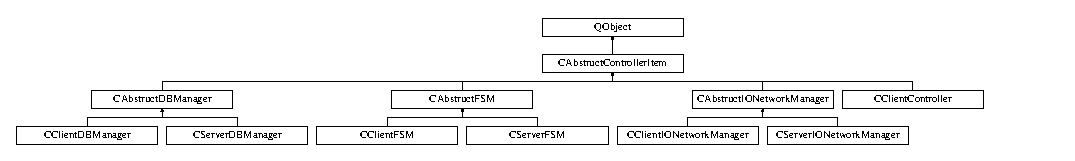
\includegraphics[height=1.720430cm]{class_c_abstruct_controller_item}
\end{center}
\end{figure}
\subsection*{Сигналы}
\begin{DoxyCompactItemize}
\item 
\hypertarget{class_c_abstruct_controller_item_a7cf2bebc87a7d0b660318e946a176eb9}{}\label{class_c_abstruct_controller_item_a7cf2bebc87a7d0b660318e946a176eb9} 
void \hyperlink{class_c_abstruct_controller_item_a7cf2bebc87a7d0b660318e946a176eb9}{send\+Data} (Q\+String $\ast$)
\begin{DoxyCompactList}\small\item\em Сигнал передачи данных внешним объектам. \end{DoxyCompactList}\item 
\hypertarget{class_c_abstruct_controller_item_a6898e48061cb0cac2065f8193bd386c1}{}\label{class_c_abstruct_controller_item_a6898e48061cb0cac2065f8193bd386c1} 
void \hyperlink{class_c_abstruct_controller_item_a6898e48061cb0cac2065f8193bd386c1}{recv\+Data} (Q\+String $\ast$)
\begin{DoxyCompactList}\small\item\em Сигнал приема данных от внешнего объекта. \end{DoxyCompactList}\end{DoxyCompactItemize}
\subsection*{Открытые члены}
\begin{DoxyCompactItemize}
\item 
\hyperlink{class_c_abstruct_controller_item_a1d99654a9522cc8721a329d1dcee35a4}{C\+Abstruct\+Controller\+Item} (Q\+Object $\ast$parent=0)
\begin{DoxyCompactList}\small\item\em Коструктор \end{DoxyCompactList}\item 
\hypertarget{class_c_abstruct_controller_item_a807bca71bd9a2966e60ec5c3c807f359}{}\label{class_c_abstruct_controller_item_a807bca71bd9a2966e60ec5c3c807f359} 
virtual \hyperlink{class_c_abstruct_controller_item_a807bca71bd9a2966e60ec5c3c807f359}{$\sim$\+C\+Abstruct\+Controller\+Item} ()
\begin{DoxyCompactList}\small\item\em Виртуальный деструктор \end{DoxyCompactList}\end{DoxyCompactItemize}
\subsection*{Защищенные члены}
\begin{DoxyCompactItemize}
\item 
\hypertarget{class_c_abstruct_controller_item_a27c6889230a86cb0782e6d7596b883c1}{}\label{class_c_abstruct_controller_item_a27c6889230a86cb0782e6d7596b883c1} 
virtual void \hyperlink{class_c_abstruct_controller_item_a27c6889230a86cb0782e6d7596b883c1}{init\+Connections} ()=0
\begin{DoxyCompactList}\small\item\em Чисто виртуальный метод необходим для инициализации сигналов и слотов d классах наследниках. \end{DoxyCompactList}\end{DoxyCompactItemize}


\subsection{Подробное описание}
Абстрактный класс задает интерфейс для взаимодействия объектов контроллера. 

Класс задает интерфейс взаимодействия объектов контроллера при помощи сигналов \hyperlink{class_c_abstruct_controller_item_a7cf2bebc87a7d0b660318e946a176eb9}{send\+Data()} и \hyperlink{class_c_abstruct_controller_item_a6898e48061cb0cac2065f8193bd386c1}{recv\+Data()}. Класс содержит чисто виртуальный метод init\+Connect() для инициализации сигналов и слотов в классах наследниках. В классах наследниках для передачи данных внешним объектам необходимо использовать сигнал \hyperlink{class_c_abstruct_controller_item_a7cf2bebc87a7d0b660318e946a176eb9}{send\+Data()}, а для приема данных от внешних объектов необходимо использовать сигнал \hyperlink{class_c_abstruct_controller_item_a6898e48061cb0cac2065f8193bd386c1}{recv\+Data()}. 

\subsection{Конструктор(ы)}
\hypertarget{class_c_abstruct_controller_item_a1d99654a9522cc8721a329d1dcee35a4}{}\label{class_c_abstruct_controller_item_a1d99654a9522cc8721a329d1dcee35a4} 
\index{C\+Abstruct\+Controller\+Item@{C\+Abstruct\+Controller\+Item}!C\+Abstruct\+Controller\+Item@{C\+Abstruct\+Controller\+Item}}
\index{C\+Abstruct\+Controller\+Item@{C\+Abstruct\+Controller\+Item}!C\+Abstruct\+Controller\+Item@{C\+Abstruct\+Controller\+Item}}
\subsubsection{\texorpdfstring{C\+Abstruct\+Controller\+Item()}{CAbstructControllerItem()}}
{\footnotesize\ttfamily C\+Abstruct\+Controller\+Item\+::\+C\+Abstruct\+Controller\+Item (\begin{DoxyParamCaption}\item[{Q\+Object $\ast$}]{parent = {\ttfamily 0} }\end{DoxyParamCaption})\hspace{0.3cm}{\ttfamily [explicit]}}



Коструктор 


\begin{DoxyParams}{Аргументы}
{\em parent} & Указатель на корневой (родительский) объект в структуре иерархии объектов \\
\hline
\end{DoxyParams}


Объявления и описания членов классов находятся в файлах\+:\begin{DoxyCompactItemize}
\item 
E\+:/workspace/\+Qt/\+Personal\+Trainer/\+Personal\+Trainer/\+Personal\+Trainer/lib/cabstructcontrolleritem.\+h\item 
E\+:/workspace/\+Qt/\+Personal\+Trainer/\+Personal\+Trainer/\+Personal\+Trainer/lib/cabstructcontrolleritem.\+cpp\end{DoxyCompactItemize}

\hypertarget{class_c_abstruct_d_b_manager}{}\section{Класс C\+Abstruct\+D\+B\+Manager}
\label{class_c_abstruct_d_b_manager}\index{C\+Abstruct\+D\+B\+Manager@{C\+Abstruct\+D\+B\+Manager}}


Базовый класс задает базовый функционал работы с базой данных.  




{\ttfamily \#include $<$cabstructdbmanager.\+h$>$}

Граф наследования\+:C\+Abstruct\+D\+B\+Manager\+:\begin{figure}[H]
\begin{center}
\leavevmode
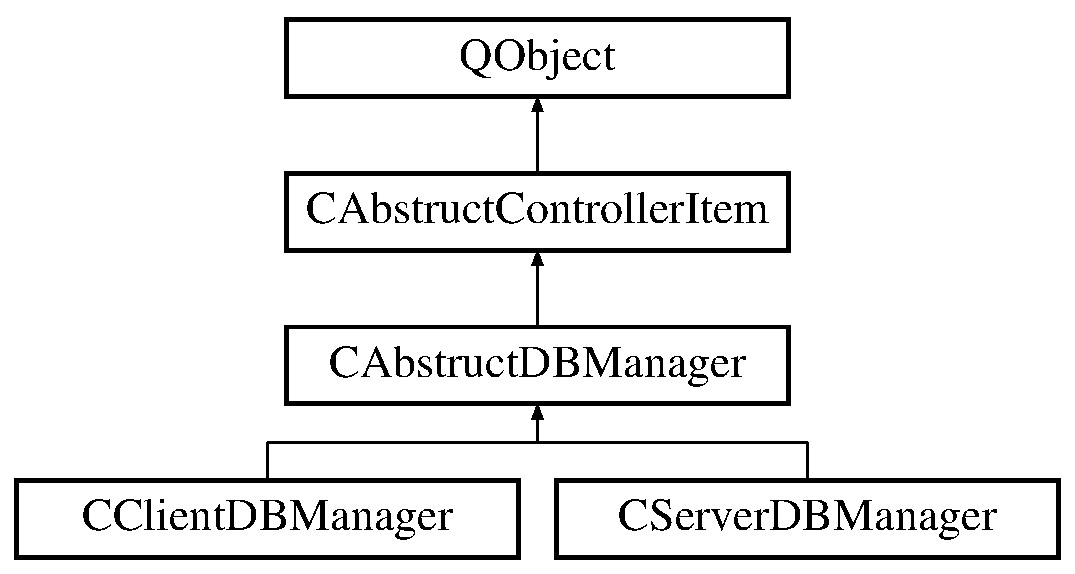
\includegraphics[height=4.000000cm]{class_c_abstruct_d_b_manager}
\end{center}
\end{figure}
\subsection*{Открытые члены}
\begin{DoxyCompactItemize}
\item 
\hyperlink{class_c_abstruct_d_b_manager_a53c2018cfa7a1a24bacd747967509bd7}{C\+Abstruct\+D\+B\+Manager} (Q\+Object $\ast$parent=0)
\begin{DoxyCompactList}\small\item\em \hyperlink{class_c_abstruct_d_b_manager}{C\+Abstruct\+D\+B\+Manager}. \end{DoxyCompactList}\item 
\hypertarget{class_c_abstruct_d_b_manager_a75785e87f1f6dcb6cc2d48d4eced257b}{}\label{class_c_abstruct_d_b_manager_a75785e87f1f6dcb6cc2d48d4eced257b} 
virtual \hyperlink{class_c_abstruct_d_b_manager_a75785e87f1f6dcb6cc2d48d4eced257b}{$\sim$\+C\+Abstruct\+D\+B\+Manager} ()
\begin{DoxyCompactList}\small\item\em $\sim$\+C\+Abstruct\+D\+B\+Manager \end{DoxyCompactList}\end{DoxyCompactItemize}
\subsection*{Защищенные члены}
\begin{DoxyCompactItemize}
\item 
\hypertarget{class_c_abstruct_d_b_manager_ad450c557df6d9a7dfcc4a37082f35659}{}\label{class_c_abstruct_d_b_manager_ad450c557df6d9a7dfcc4a37082f35659} 
void \hyperlink{class_c_abstruct_d_b_manager_ad450c557df6d9a7dfcc4a37082f35659}{init\+Connections} ()
\begin{DoxyCompactList}\small\item\em Реализация виртуального метода базового класса. \end{DoxyCompactList}\end{DoxyCompactItemize}
\subsection*{Дополнительные унаследованные члены}


\subsection{Подробное описание}
Базовый класс задает базовый функционал работы с базой данных. 

\subsection{Конструктор(ы)}
\hypertarget{class_c_abstruct_d_b_manager_a53c2018cfa7a1a24bacd747967509bd7}{}\label{class_c_abstruct_d_b_manager_a53c2018cfa7a1a24bacd747967509bd7} 
\index{C\+Abstruct\+D\+B\+Manager@{C\+Abstruct\+D\+B\+Manager}!C\+Abstruct\+D\+B\+Manager@{C\+Abstruct\+D\+B\+Manager}}
\index{C\+Abstruct\+D\+B\+Manager@{C\+Abstruct\+D\+B\+Manager}!C\+Abstruct\+D\+B\+Manager@{C\+Abstruct\+D\+B\+Manager}}
\subsubsection{\texorpdfstring{C\+Abstruct\+D\+B\+Manager()}{CAbstructDBManager()}}
{\footnotesize\ttfamily C\+Abstruct\+D\+B\+Manager\+::\+C\+Abstruct\+D\+B\+Manager (\begin{DoxyParamCaption}\item[{Q\+Object $\ast$}]{parent = {\ttfamily 0} }\end{DoxyParamCaption})\hspace{0.3cm}{\ttfamily [explicit]}}



\hyperlink{class_c_abstruct_d_b_manager}{C\+Abstruct\+D\+B\+Manager}. 


\begin{DoxyParams}{Аргументы}
{\em parent} & \\
\hline
\end{DoxyParams}


Объявления и описания членов классов находятся в файлах\+:\begin{DoxyCompactItemize}
\item 
E\+:/workspace/\+Qt/\+Personal\+Trainer/\+Personal\+Trainer/\+Personal\+Trainer/lib/cabstructdbmanager.\+h\item 
E\+:/workspace/\+Qt/\+Personal\+Trainer/\+Personal\+Trainer/\+Personal\+Trainer/lib/cabstructdbmanager.\+cpp\end{DoxyCompactItemize}

\hypertarget{class_c_abstruct_f_s_m}{}\section{Класс C\+Abstruct\+F\+SM}
\label{class_c_abstruct_f_s_m}\index{C\+Abstruct\+F\+SM@{C\+Abstruct\+F\+SM}}


Базовый класс реализующий базовый функционал конечного автомата.  




{\ttfamily \#include $<$cabstructfsm.\+h$>$}

Граф наследования\+:C\+Abstruct\+F\+SM\+:\begin{figure}[H]
\begin{center}
\leavevmode
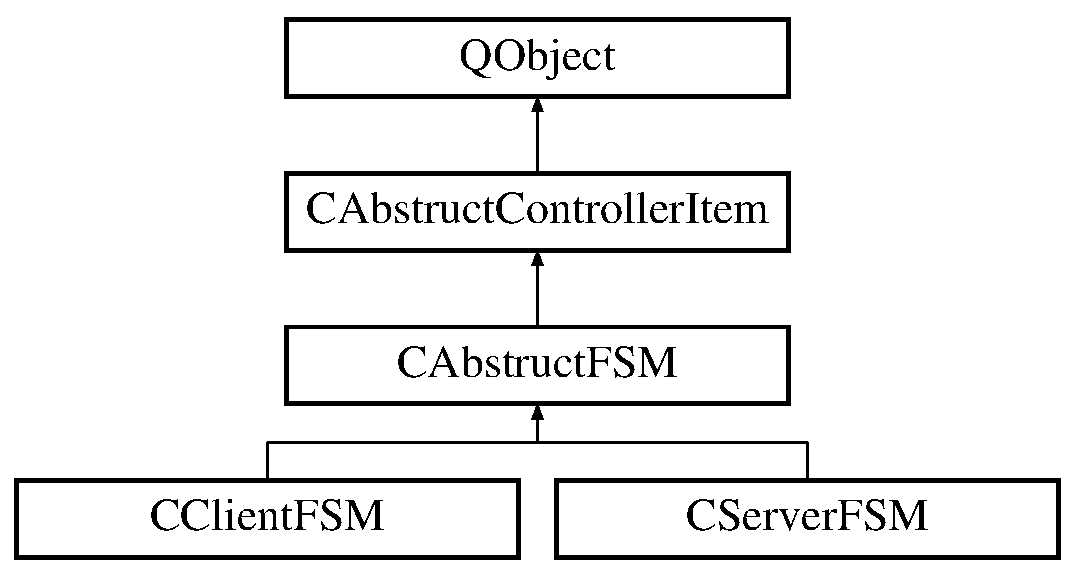
\includegraphics[height=4.000000cm]{class_c_abstruct_f_s_m}
\end{center}
\end{figure}
\subsection*{Открытые слоты}
\begin{DoxyCompactItemize}
\item 
void \hyperlink{class_c_abstruct_f_s_m_ae06497e1f93385cd6c20eaa84fc253c1}{fsm} (Q\+String $\ast$data)
\begin{DoxyCompactList}\small\item\em Базовый функционал конечного автомата. \end{DoxyCompactList}\end{DoxyCompactItemize}
\subsection*{Сигналы}
\begin{DoxyCompactItemize}
\item 
void \hyperlink{class_c_abstruct_f_s_m_a542570a7469e3923eeace7c3c308ff97}{send\+Data\+To\+I\+O\+Network\+Manager} (Q\+String $\ast$)
\begin{DoxyCompactList}\small\item\em Сигнал передачи данных объекту управляющему сетевым взаимодействием. \end{DoxyCompactList}\item 
void \hyperlink{class_c_abstruct_f_s_m_a8b3e4a9134df07825f357d16e6d7c436}{send\+Data\+To\+D\+B\+Manager} (Q\+String $\ast$)
\begin{DoxyCompactList}\small\item\em Сигнал передачи данных объекту работающему с базой данных. \end{DoxyCompactList}\end{DoxyCompactItemize}
\subsection*{Открытые члены}
\begin{DoxyCompactItemize}
\item 
\hyperlink{class_c_abstruct_f_s_m_a54037c986f6b437c50d5e8ba42063330}{C\+Abstruct\+F\+SM} (Q\+Object $\ast$parent=0)
\begin{DoxyCompactList}\small\item\em \hyperlink{class_c_abstruct_f_s_m_a54037c986f6b437c50d5e8ba42063330}{C\+Abstruct\+F\+S\+M\+::\+C\+Abstruct\+F\+SM}. \end{DoxyCompactList}\item 
virtual \hyperlink{class_c_abstruct_f_s_m_acef4a425dee5b9705bc6bbff79225bae}{$\sim$\+C\+Abstruct\+F\+SM} ()
\begin{DoxyCompactList}\small\item\em \hyperlink{class_c_abstruct_f_s_m_acef4a425dee5b9705bc6bbff79225bae}{C\+Abstruct\+F\+S\+M\+::$\sim$\+C\+Abstruct\+F\+SM}. \end{DoxyCompactList}\end{DoxyCompactItemize}
\subsection*{Защищенные члены}
\begin{DoxyCompactItemize}
\item 
void \hyperlink{class_c_abstruct_f_s_m_a9d6f4659a08f3028f8c047243f8dcfc3}{init\+Connections} ()
\begin{DoxyCompactList}\small\item\em Реализация виртуального метода базового класса. Устанавливает связь между принимаемыми данными от сигнала \hyperlink{class_c_abstruct_controller_item_a6898e48061cb0cac2065f8193bd386c1}{recv\+Data()} и слотом \hyperlink{class_c_abstruct_f_s_m_ae06497e1f93385cd6c20eaa84fc253c1}{fsm()} \end{DoxyCompactList}\end{DoxyCompactItemize}


\subsection{Подробное описание}
Базовый класс реализующий базовый функционал конечного автомата. 

См. определение в файле cabstructfsm.\+h строка 12



\subsection{Конструктор(ы)}
\hypertarget{class_c_abstruct_f_s_m_a54037c986f6b437c50d5e8ba42063330}{}\label{class_c_abstruct_f_s_m_a54037c986f6b437c50d5e8ba42063330} 
\index{C\+Abstruct\+F\+SM@{C\+Abstruct\+F\+SM}!C\+Abstruct\+F\+SM@{C\+Abstruct\+F\+SM}}
\index{C\+Abstruct\+F\+SM@{C\+Abstruct\+F\+SM}!C\+Abstruct\+F\+SM@{C\+Abstruct\+F\+SM}}
\subsubsection{\texorpdfstring{C\+Abstruct\+F\+S\+M()}{CAbstructFSM()}}
{\footnotesize\ttfamily C\+Abstruct\+F\+S\+M\+::\+C\+Abstruct\+F\+SM (\begin{DoxyParamCaption}\item[{Q\+Object $\ast$}]{parent = {\ttfamily 0} }\end{DoxyParamCaption})\hspace{0.3cm}{\ttfamily [explicit]}}



\hyperlink{class_c_abstruct_f_s_m_a54037c986f6b437c50d5e8ba42063330}{C\+Abstruct\+F\+S\+M\+::\+C\+Abstruct\+F\+SM}. 


\begin{DoxyParams}{Аргументы}
{\em parent} & В конструкторе вызывается метод \hyperlink{class_c_abstruct_f_s_m_a9d6f4659a08f3028f8c047243f8dcfc3}{init\+Connections()}; \\
\hline
\end{DoxyParams}


См. определение в файле cabstructfsm.\+cpp строка 9



Перекрестные ссылки init\+Connections().


\begin{DoxyCode}
9                                           :
10     \hyperlink{class_c_abstruct_controller_item_a1d99654a9522cc8721a329d1dcee35a4}{CAbstructControllerItem}(parent)
11 \{
12     \hyperlink{class_c_abstruct_f_s_m_a9d6f4659a08f3028f8c047243f8dcfc3}{initConnections}();
13 \}
\end{DoxyCode}
\hypertarget{class_c_abstruct_f_s_m_acef4a425dee5b9705bc6bbff79225bae}{}\label{class_c_abstruct_f_s_m_acef4a425dee5b9705bc6bbff79225bae} 
\index{C\+Abstruct\+F\+SM@{C\+Abstruct\+F\+SM}!````~C\+Abstruct\+F\+SM@{$\sim$\+C\+Abstruct\+F\+SM}}
\index{````~C\+Abstruct\+F\+SM@{$\sim$\+C\+Abstruct\+F\+SM}!C\+Abstruct\+F\+SM@{C\+Abstruct\+F\+SM}}
\subsubsection{\texorpdfstring{$\sim$\+C\+Abstruct\+F\+S\+M()}{~CAbstructFSM()}}
{\footnotesize\ttfamily C\+Abstruct\+F\+S\+M\+::$\sim$\+C\+Abstruct\+F\+SM (\begin{DoxyParamCaption}{ }\end{DoxyParamCaption})\hspace{0.3cm}{\ttfamily [virtual]}}



\hyperlink{class_c_abstruct_f_s_m_acef4a425dee5b9705bc6bbff79225bae}{C\+Abstruct\+F\+S\+M\+::$\sim$\+C\+Abstruct\+F\+SM}. 



См. определение в файле cabstructfsm.\+cpp строка 18


\begin{DoxyCode}
19 \{
20     qDebug() << \textcolor{stringliteral}{"CAbsrtuctFSM: destructor "} << \textcolor{keyword}{this};
21 \}
\end{DoxyCode}


\subsection{Методы}
\hypertarget{class_c_abstruct_f_s_m_ae06497e1f93385cd6c20eaa84fc253c1}{}\label{class_c_abstruct_f_s_m_ae06497e1f93385cd6c20eaa84fc253c1} 
\index{C\+Abstruct\+F\+SM@{C\+Abstruct\+F\+SM}!fsm@{fsm}}
\index{fsm@{fsm}!C\+Abstruct\+F\+SM@{C\+Abstruct\+F\+SM}}
\subsubsection{\texorpdfstring{fsm}{fsm}}
{\footnotesize\ttfamily void C\+Abstruct\+F\+S\+M\+::fsm (\begin{DoxyParamCaption}\item[{Q\+String $\ast$}]{data }\end{DoxyParamCaption})\hspace{0.3cm}{\ttfamily [slot]}}



Базовый функционал конечного автомата. 


\begin{DoxyParams}{Аргументы}
{\em data} & Принимаемые данные \\
\hline
\end{DoxyParams}


См. определение в файле cabstructfsm.\+cpp строка 28



Перекрестные ссылки send\+Data\+To\+I\+O\+Network\+Manager().



Используется в init\+Connections().


\begin{DoxyCode}
29 \{
30     qDebug() << *data;
31     emit \hyperlink{class_c_abstruct_f_s_m_a542570a7469e3923eeace7c3c308ff97}{sendDataToIONetworkManager}(\textcolor{keyword}{new} QString(*data));
32     \textcolor{keyword}{delete} data;
33 \}
\end{DoxyCode}
\hypertarget{class_c_abstruct_f_s_m_a9d6f4659a08f3028f8c047243f8dcfc3}{}\label{class_c_abstruct_f_s_m_a9d6f4659a08f3028f8c047243f8dcfc3} 
\index{C\+Abstruct\+F\+SM@{C\+Abstruct\+F\+SM}!init\+Connections@{init\+Connections}}
\index{init\+Connections@{init\+Connections}!C\+Abstruct\+F\+SM@{C\+Abstruct\+F\+SM}}
\subsubsection{\texorpdfstring{init\+Connections()}{initConnections()}}
{\footnotesize\ttfamily void C\+Abstruct\+F\+S\+M\+::init\+Connections (\begin{DoxyParamCaption}{ }\end{DoxyParamCaption})\hspace{0.3cm}{\ttfamily [protected]}, {\ttfamily [virtual]}}



Реализация виртуального метода базового класса. Устанавливает связь между принимаемыми данными от сигнала \hyperlink{class_c_abstruct_controller_item_a6898e48061cb0cac2065f8193bd386c1}{recv\+Data()} и слотом \hyperlink{class_c_abstruct_f_s_m_ae06497e1f93385cd6c20eaa84fc253c1}{fsm()} 



Замещает \hyperlink{class_c_abstruct_controller_item_a27c6889230a86cb0782e6d7596b883c1}{C\+Abstruct\+Controller\+Item}.



Переопределяется в \hyperlink{class_c_server_f_s_m_ae0e6a994505c26e60b718af9989bea77}{C\+Server\+F\+SM}.



См. определение в файле cabstructfsm.\+cpp строка 40



Перекрестные ссылки fsm() и C\+Abstruct\+Controller\+Item\+::recv\+Data().



Используется в C\+Abstruct\+F\+S\+M().


\begin{DoxyCode}
41 \{
42     connect(\textcolor{keyword}{this}, SIGNAL(\hyperlink{class_c_abstruct_controller_item_a6898e48061cb0cac2065f8193bd386c1}{recvData}(QString*)), SLOT(\hyperlink{class_c_abstruct_f_s_m_ae06497e1f93385cd6c20eaa84fc253c1}{fsm}(QString*)));
43 \}
\end{DoxyCode}
\hypertarget{class_c_abstruct_f_s_m_a8b3e4a9134df07825f357d16e6d7c436}{}\label{class_c_abstruct_f_s_m_a8b3e4a9134df07825f357d16e6d7c436} 
\index{C\+Abstruct\+F\+SM@{C\+Abstruct\+F\+SM}!send\+Data\+To\+D\+B\+Manager@{send\+Data\+To\+D\+B\+Manager}}
\index{send\+Data\+To\+D\+B\+Manager@{send\+Data\+To\+D\+B\+Manager}!C\+Abstruct\+F\+SM@{C\+Abstruct\+F\+SM}}
\subsubsection{\texorpdfstring{send\+Data\+To\+D\+B\+Manager}{sendDataToDBManager}}
{\footnotesize\ttfamily void C\+Abstruct\+F\+S\+M\+::send\+Data\+To\+D\+B\+Manager (\begin{DoxyParamCaption}\item[{Q\+String $\ast$}]{ }\end{DoxyParamCaption})\hspace{0.3cm}{\ttfamily [signal]}}



Сигнал передачи данных объекту работающему с базой данных. 

\hypertarget{class_c_abstruct_f_s_m_a542570a7469e3923eeace7c3c308ff97}{}\label{class_c_abstruct_f_s_m_a542570a7469e3923eeace7c3c308ff97} 
\index{C\+Abstruct\+F\+SM@{C\+Abstruct\+F\+SM}!send\+Data\+To\+I\+O\+Network\+Manager@{send\+Data\+To\+I\+O\+Network\+Manager}}
\index{send\+Data\+To\+I\+O\+Network\+Manager@{send\+Data\+To\+I\+O\+Network\+Manager}!C\+Abstruct\+F\+SM@{C\+Abstruct\+F\+SM}}
\subsubsection{\texorpdfstring{send\+Data\+To\+I\+O\+Network\+Manager}{sendDataToIONetworkManager}}
{\footnotesize\ttfamily void C\+Abstruct\+F\+S\+M\+::send\+Data\+To\+I\+O\+Network\+Manager (\begin{DoxyParamCaption}\item[{Q\+String $\ast$}]{ }\end{DoxyParamCaption})\hspace{0.3cm}{\ttfamily [signal]}}



Сигнал передачи данных объекту управляющему сетевым взаимодействием. 



Используется в fsm().



Объявления и описания членов классов находятся в файлах\+:\begin{DoxyCompactItemize}
\item 
lib/\hyperlink{cabstructfsm_8h}{cabstructfsm.\+h}\item 
lib/\hyperlink{cabstructfsm_8cpp}{cabstructfsm.\+cpp}\end{DoxyCompactItemize}

\hypertarget{class_c_abstruct_i_o_network_manager}{}\section{Класс C\+Abstruct\+I\+O\+Network\+Manager}
\label{class_c_abstruct_i_o_network_manager}\index{C\+Abstruct\+I\+O\+Network\+Manager@{C\+Abstruct\+I\+O\+Network\+Manager}}


Базовый класс передачи и приема данных по сети.  




{\ttfamily \#include $<$cabstructionetworkmanager.\+h$>$}

Граф наследования\+:C\+Abstruct\+I\+O\+Network\+Manager\+:\begin{figure}[H]
\begin{center}
\leavevmode
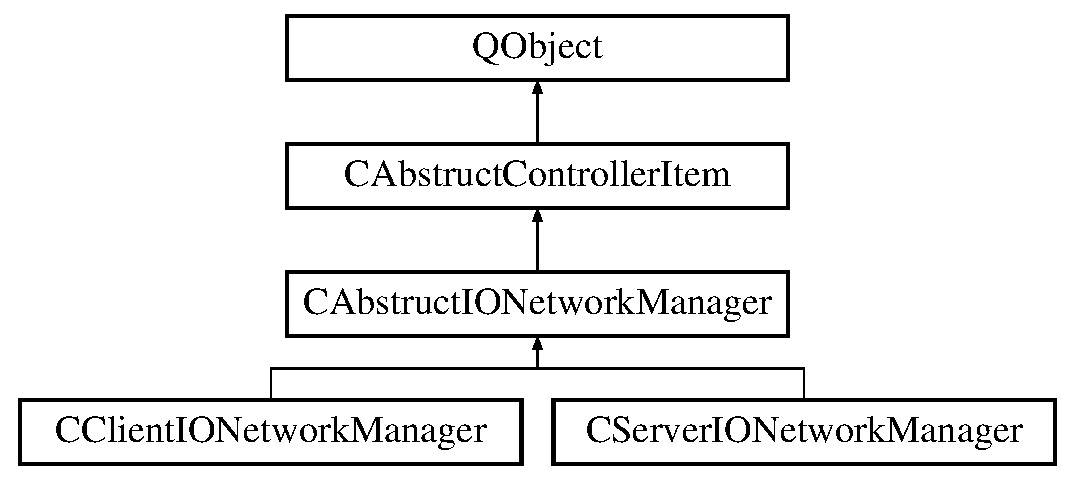
\includegraphics[height=4.000000cm]{class_c_abstruct_i_o_network_manager}
\end{center}
\end{figure}
\subsection*{Открытые слоты}
\begin{DoxyCompactItemize}
\item 
void \hyperlink{class_c_abstruct_i_o_network_manager_a78756fc08ed619162da210a9cfc09208}{recv\+Data\+From\+Socket} ()
\begin{DoxyCompactList}\small\item\em Слот приема данных по сети \end{DoxyCompactList}\item 
void \hyperlink{class_c_abstruct_i_o_network_manager_a7e6c20ce1264c76a2cc66114f8490629}{send\+Data\+To\+Socket} (Q\+String $\ast$data)
\begin{DoxyCompactList}\small\item\em Слот передачи данных по сети \end{DoxyCompactList}\end{DoxyCompactItemize}
\subsection*{Сигналы}
\begin{DoxyCompactItemize}
\item 
\hypertarget{class_c_abstruct_i_o_network_manager_a4c25afd753612c5c719944a3e8ef4373}{}\label{class_c_abstruct_i_o_network_manager_a4c25afd753612c5c719944a3e8ef4373} 
void \hyperlink{class_c_abstruct_i_o_network_manager_a4c25afd753612c5c719944a3e8ef4373}{disconnected} ()
\begin{DoxyCompactList}\small\item\em Сигнал генерируется когда сокет генерирует сигнал disconected() \end{DoxyCompactList}\end{DoxyCompactItemize}
\subsection*{Открытые члены}
\begin{DoxyCompactItemize}
\item 
\hyperlink{class_c_abstruct_i_o_network_manager_a4ed201a3712ddf4ccd2135a0eb40fbf2}{C\+Abstruct\+I\+O\+Network\+Manager} (Q\+Tcp\+Socket $\ast$socket, Q\+Object $\ast$parent=0)
\begin{DoxyCompactList}\small\item\em Коструктор \end{DoxyCompactList}\item 
\hypertarget{class_c_abstruct_i_o_network_manager_ae6a3817e290e0ff8fcbf3d4c6830f5cd}{}\label{class_c_abstruct_i_o_network_manager_ae6a3817e290e0ff8fcbf3d4c6830f5cd} 
virtual \hyperlink{class_c_abstruct_i_o_network_manager_ae6a3817e290e0ff8fcbf3d4c6830f5cd}{$\sim$\+C\+Abstruct\+I\+O\+Network\+Manager} ()
\begin{DoxyCompactList}\small\item\em Деструктор \end{DoxyCompactList}\item 
Q\+Tcp\+Socket $\ast$ \hyperlink{class_c_abstruct_i_o_network_manager_a118a2c8254c149614cba51c42147c709}{get\+Socket} () const
\begin{DoxyCompactList}\small\item\em Функиция-\/getter для сокета \end{DoxyCompactList}\end{DoxyCompactItemize}
\subsection*{Защищенные члены}
\begin{DoxyCompactItemize}
\item 
void \hyperlink{class_c_abstruct_i_o_network_manager_ac01bfefacfa37050c8d3a9317a38fbf5}{init\+Connections} ()
\begin{DoxyCompactList}\small\item\em Инициализация подключений сигналов и слотов \end{DoxyCompactList}\end{DoxyCompactItemize}


\subsection{Подробное описание}
Базовый класс передачи и приема данных по сети. 

\subsection{Конструктор(ы)}
\hypertarget{class_c_abstruct_i_o_network_manager_a4ed201a3712ddf4ccd2135a0eb40fbf2}{}\label{class_c_abstruct_i_o_network_manager_a4ed201a3712ddf4ccd2135a0eb40fbf2} 
\index{C\+Abstruct\+I\+O\+Network\+Manager@{C\+Abstruct\+I\+O\+Network\+Manager}!C\+Abstruct\+I\+O\+Network\+Manager@{C\+Abstruct\+I\+O\+Network\+Manager}}
\index{C\+Abstruct\+I\+O\+Network\+Manager@{C\+Abstruct\+I\+O\+Network\+Manager}!C\+Abstruct\+I\+O\+Network\+Manager@{C\+Abstruct\+I\+O\+Network\+Manager}}
\subsubsection{\texorpdfstring{C\+Abstruct\+I\+O\+Network\+Manager()}{CAbstructIONetworkManager()}}
{\footnotesize\ttfamily C\+Abstruct\+I\+O\+Network\+Manager\+::\+C\+Abstruct\+I\+O\+Network\+Manager (\begin{DoxyParamCaption}\item[{Q\+Tcp\+Socket $\ast$}]{socket,  }\item[{Q\+Object $\ast$}]{parent = {\ttfamily 0} }\end{DoxyParamCaption})\hspace{0.3cm}{\ttfamily [explicit]}}



Коструктор 


\begin{DoxyParams}[1]{Аргументы}
\mbox{\tt in}  & {\em socket} & Сокет работы с сетью. \\
\hline
\mbox{\tt in}  & {\em parent} & Объект верхнего уровня иерархии объектов \\
\hline
\end{DoxyParams}


\subsection{Методы}
\hypertarget{class_c_abstruct_i_o_network_manager_a118a2c8254c149614cba51c42147c709}{}\label{class_c_abstruct_i_o_network_manager_a118a2c8254c149614cba51c42147c709} 
\index{C\+Abstruct\+I\+O\+Network\+Manager@{C\+Abstruct\+I\+O\+Network\+Manager}!get\+Socket@{get\+Socket}}
\index{get\+Socket@{get\+Socket}!C\+Abstruct\+I\+O\+Network\+Manager@{C\+Abstruct\+I\+O\+Network\+Manager}}
\subsubsection{\texorpdfstring{get\+Socket()}{getSocket()}}
{\footnotesize\ttfamily Q\+Tcp\+Socket $\ast$ C\+Abstruct\+I\+O\+Network\+Manager\+::get\+Socket (\begin{DoxyParamCaption}{ }\end{DoxyParamCaption}) const}



Функиция-\/getter для сокета 

\begin{DoxyReturn}{Возвращает}
Возвращает указатель на сокет 
\end{DoxyReturn}
\hypertarget{class_c_abstruct_i_o_network_manager_ac01bfefacfa37050c8d3a9317a38fbf5}{}\label{class_c_abstruct_i_o_network_manager_ac01bfefacfa37050c8d3a9317a38fbf5} 
\index{C\+Abstruct\+I\+O\+Network\+Manager@{C\+Abstruct\+I\+O\+Network\+Manager}!init\+Connections@{init\+Connections}}
\index{init\+Connections@{init\+Connections}!C\+Abstruct\+I\+O\+Network\+Manager@{C\+Abstruct\+I\+O\+Network\+Manager}}
\subsubsection{\texorpdfstring{init\+Connections()}{initConnections()}}
{\footnotesize\ttfamily void C\+Abstruct\+I\+O\+Network\+Manager\+::init\+Connections (\begin{DoxyParamCaption}{ }\end{DoxyParamCaption})\hspace{0.3cm}{\ttfamily [protected]}, {\ttfamily [virtual]}}



Инициализация подключений сигналов и слотов 

Соединяем сигнал сокета ready\+Read() и слот \hyperlink{class_c_abstruct_i_o_network_manager_a78756fc08ed619162da210a9cfc09208}{C\+Abstruct\+I\+O\+Network\+Manager\+::recv\+Data\+From\+Socket()}.  Когда сокет генерирует сигнал ready\+Read(), т.\+е. сокету отправили из сети данные, которые он готов принять, вызывется слот приема данных из сети

Замещает \hyperlink{class_c_abstruct_controller_item_a27c6889230a86cb0782e6d7596b883c1}{C\+Abstruct\+Controller\+Item}.



Переопределяется в \hyperlink{class_c_server_i_o_network_manager_a17155570c51dc951db52d827f120c689}{C\+Server\+I\+O\+Network\+Manager}.

\hypertarget{class_c_abstruct_i_o_network_manager_a78756fc08ed619162da210a9cfc09208}{}\label{class_c_abstruct_i_o_network_manager_a78756fc08ed619162da210a9cfc09208} 
\index{C\+Abstruct\+I\+O\+Network\+Manager@{C\+Abstruct\+I\+O\+Network\+Manager}!recv\+Data\+From\+Socket@{recv\+Data\+From\+Socket}}
\index{recv\+Data\+From\+Socket@{recv\+Data\+From\+Socket}!C\+Abstruct\+I\+O\+Network\+Manager@{C\+Abstruct\+I\+O\+Network\+Manager}}
\subsubsection{\texorpdfstring{recv\+Data\+From\+Socket}{recvDataFromSocket}}
{\footnotesize\ttfamily void C\+Abstruct\+I\+O\+Network\+Manager\+::recv\+Data\+From\+Socket (\begin{DoxyParamCaption}{ }\end{DoxyParamCaption})\hspace{0.3cm}{\ttfamily [slot]}}



Слот приема данных по сети 

Создается объект raw\+\_\+data класса Q\+Byte\+Array в который хранит данные переданные через сеть. Считывание данных происходит через вызов метода read\+All() у сокета. Массив байт помещается в объект класса Q\+String. Далее происходит генерация сигнала \hyperlink{class_c_abstruct_controller_item_a7cf2bebc87a7d0b660318e946a176eb9}{send\+Data()}. В сигнал помещается объект класса Q\+String, который содержит массив принятых байт по сети, который передается внешнему объекту. \hypertarget{class_c_abstruct_i_o_network_manager_a7e6c20ce1264c76a2cc66114f8490629}{}\label{class_c_abstruct_i_o_network_manager_a7e6c20ce1264c76a2cc66114f8490629} 
\index{C\+Abstruct\+I\+O\+Network\+Manager@{C\+Abstruct\+I\+O\+Network\+Manager}!send\+Data\+To\+Socket@{send\+Data\+To\+Socket}}
\index{send\+Data\+To\+Socket@{send\+Data\+To\+Socket}!C\+Abstruct\+I\+O\+Network\+Manager@{C\+Abstruct\+I\+O\+Network\+Manager}}
\subsubsection{\texorpdfstring{send\+Data\+To\+Socket}{sendDataToSocket}}
{\footnotesize\ttfamily void C\+Abstruct\+I\+O\+Network\+Manager\+::send\+Data\+To\+Socket (\begin{DoxyParamCaption}\item[{Q\+String $\ast$}]{data }\end{DoxyParamCaption})\hspace{0.3cm}{\ttfamily [slot]}}



Слот передачи данных по сети 


\begin{DoxyParams}[1]{Аргументы}
\mbox{\tt in}  & {\em data} & Объект содержащий передаваемую информацию\\
\hline
\end{DoxyParams}
Формируется char$\ast$ строка из переданного в слок объекта Q\+String. Для передачи данных по сети из объекта сокета вызывается метод write в который передается char$\ast$ строка и размер этой строки. Далее для ожидания передачи данных вызывается метод wait\+For\+Bytes\+Written() и очищается буффер сокета. 

Объявления и описания членов классов находятся в файлах\+:\begin{DoxyCompactItemize}
\item 
E\+:/workspace/\+Qt/\+Personal\+Trainer/\+Personal\+Trainer/\+Personal\+Trainer/lib/cabstructionetworkmanager.\+h\item 
E\+:/workspace/\+Qt/\+Personal\+Trainer/\+Personal\+Trainer/\+Personal\+Trainer/lib/cabstructionetworkmanager.\+cpp\end{DoxyCompactItemize}

\hypertarget{class_c_client_controller}{}\section{Класс C\+Client\+Controller}
\label{class_c_client_controller}\index{C\+Client\+Controller@{C\+Client\+Controller}}
Граф наследования\+:C\+Client\+Controller\+:\begin{figure}[H]
\begin{center}
\leavevmode
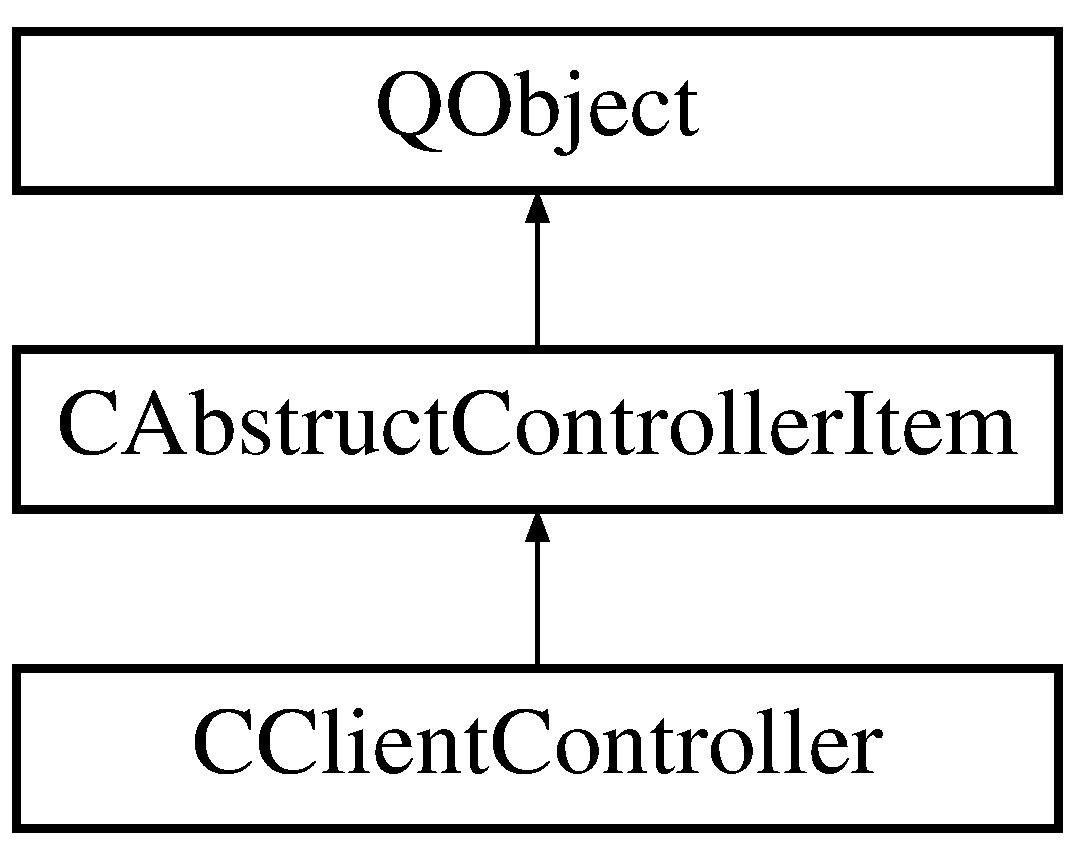
\includegraphics[height=3.000000cm]{class_c_client_controller}
\end{center}
\end{figure}
\subsection*{Сигналы}
\begin{DoxyCompactItemize}
\item 
\hypertarget{class_c_client_controller_a171db18126ffb9541f47aec5cc0eda79}{}\label{class_c_client_controller_a171db18126ffb9541f47aec5cc0eda79} 
void {\bfseries disconnected} ()
\item 
\hypertarget{class_c_client_controller_a04a024fdb1135b1b5dec86b006511672}{}\label{class_c_client_controller_a04a024fdb1135b1b5dec86b006511672} 
void {\bfseries finished} ()
\item 
\hypertarget{class_c_client_controller_a358ef743560d560acef69e90dfaca11e}{}\label{class_c_client_controller_a358ef743560d560acef69e90dfaca11e} 
void {\bfseries connect\+To\+Host} ()
\end{DoxyCompactItemize}
\subsection*{Открытые члены}
\begin{DoxyCompactItemize}
\item 
\hypertarget{class_c_client_controller_a95dd0dfe547a620dee2ae10790dee6be}{}\label{class_c_client_controller_a95dd0dfe547a620dee2ae10790dee6be} 
{\bfseries C\+Client\+Controller} (Q\+Tcp\+Socket $\ast$socket, Q\+Object $\ast$parent=0)
\item 
\hypertarget{class_c_client_controller_ab39fa71b009189acc06aa759d636de4d}{}\label{class_c_client_controller_ab39fa71b009189acc06aa759d636de4d} 
\hyperlink{class_c_client_i_o_network_manager}{C\+Client\+I\+O\+Network\+Manager} $\ast$ {\bfseries get\+I\+O\+Network\+Manager} () const
\item 
\hypertarget{class_c_client_controller_a07441870867b13d7c867e57244101f92}{}\label{class_c_client_controller_a07441870867b13d7c867e57244101f92} 
\hyperlink{class_c_client_f_s_m}{C\+Client\+F\+SM} $\ast$ {\bfseries get\+F\+SM} () const
\item 
\hypertarget{class_c_client_controller_a456359547ec2e4225d54daeb6463008b}{}\label{class_c_client_controller_a456359547ec2e4225d54daeb6463008b} 
\hyperlink{class_c_client_d_b_manager}{C\+Client\+D\+B\+Manager} $\ast$ {\bfseries get\+D\+B\+Manager} () const
\end{DoxyCompactItemize}
\subsection*{Защищенные члены}
\begin{DoxyCompactItemize}
\item 
\hypertarget{class_c_client_controller_a1dabfbc538daf66f1c2565808bc7db6d}{}\label{class_c_client_controller_a1dabfbc538daf66f1c2565808bc7db6d} 
void \hyperlink{class_c_client_controller_a1dabfbc538daf66f1c2565808bc7db6d}{init\+Connections} ()
\begin{DoxyCompactList}\small\item\em Чисто виртуальный метод необходим для инициализации сигналов и слотов d классах наследниках. \end{DoxyCompactList}\end{DoxyCompactItemize}


Объявления и описания членов классов находятся в файлах\+:\begin{DoxyCompactItemize}
\item 
E\+:/workspace/\+Qt/\+Personal\+Trainer/\+Personal\+Trainer/\+Personal\+Trainer/\+Client/cclientcontroller.\+h\item 
E\+:/workspace/\+Qt/\+Personal\+Trainer/\+Personal\+Trainer/\+Personal\+Trainer/\+Client/cclientcontroller.\+cpp\end{DoxyCompactItemize}

\hypertarget{class_c_client_d_b_manager}{}\section{Класс C\+Client\+D\+B\+Manager}
\label{class_c_client_d_b_manager}\index{C\+Client\+D\+B\+Manager@{C\+Client\+D\+B\+Manager}}


{\ttfamily \#include $<$cclientdbmanager.\+h$>$}

Граф наследования\+:C\+Client\+D\+B\+Manager\+:\begin{figure}[H]
\begin{center}
\leavevmode
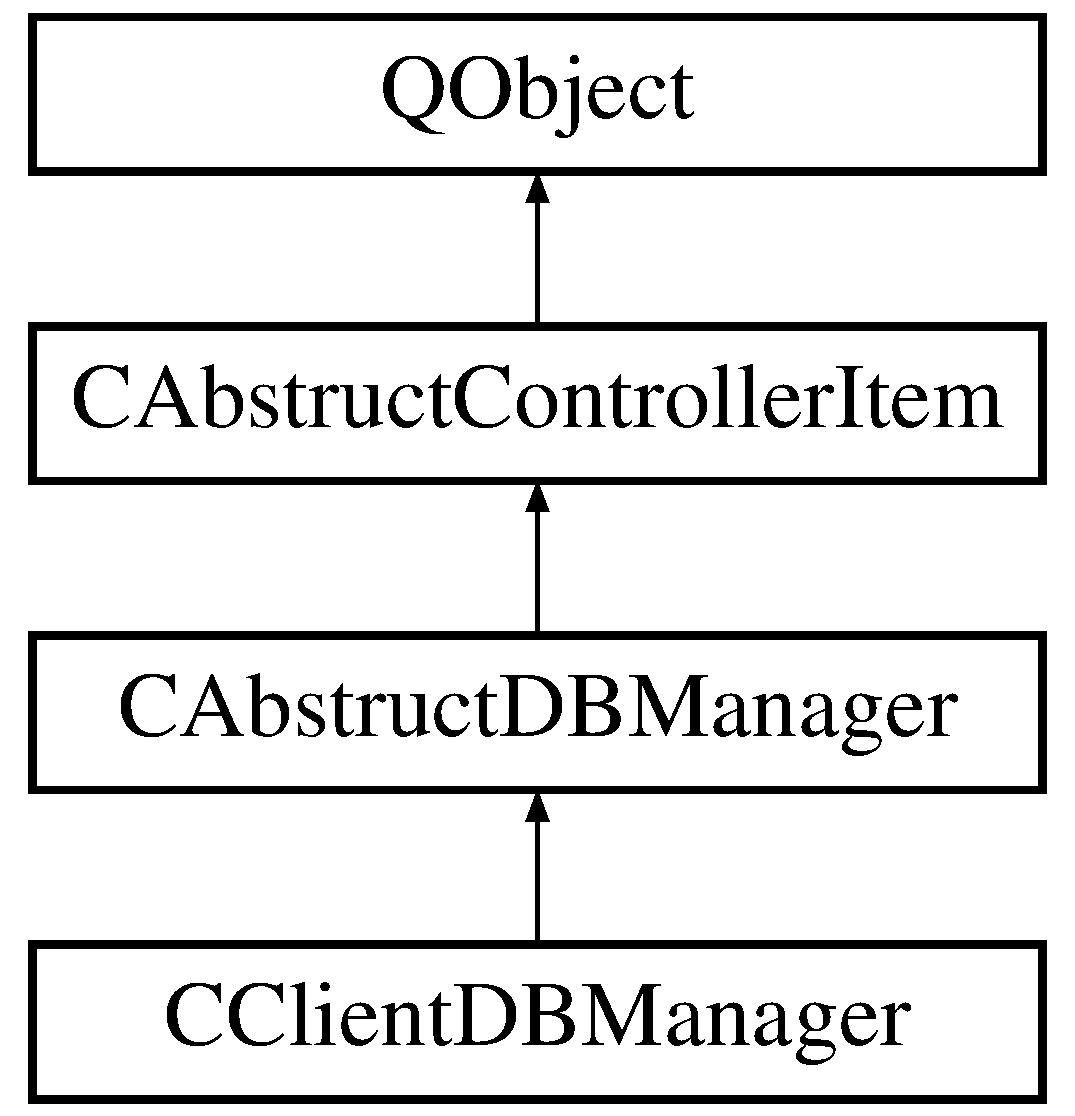
\includegraphics[height=4.000000cm]{class_c_client_d_b_manager}
\end{center}
\end{figure}
\subsection*{Открытые члены}
\begin{DoxyCompactItemize}
\item 
\hyperlink{class_c_client_d_b_manager_aaac2c483f7a445d8565a6dd35f1a77b9}{C\+Client\+D\+B\+Manager} (Q\+Object $\ast$parent=0)
\item 
virtual \hyperlink{class_c_client_d_b_manager_a93ee522535ebb3bcba938b251ee9fa1b}{$\sim$\+C\+Client\+D\+B\+Manager} ()
\end{DoxyCompactItemize}
\subsection*{Защищенные члены}
\begin{DoxyCompactItemize}
\item 
void \hyperlink{class_c_client_d_b_manager_a85d962d6f61d8f9480b6bc9a7f121204}{init\+Connections} ()
\begin{DoxyCompactList}\small\item\em Чисто виртуальный метод необходим для инициализации сигналов и слотов d классах наследниках. \end{DoxyCompactList}\end{DoxyCompactItemize}
\subsection*{Дополнительные унаследованные члены}


\subsection{Подробное описание}


См. определение в файле cclientdbmanager.\+h строка 7



\subsection{Конструктор(ы)}
\hypertarget{class_c_client_d_b_manager_aaac2c483f7a445d8565a6dd35f1a77b9}{}\label{class_c_client_d_b_manager_aaac2c483f7a445d8565a6dd35f1a77b9} 
\index{C\+Client\+D\+B\+Manager@{C\+Client\+D\+B\+Manager}!C\+Client\+D\+B\+Manager@{C\+Client\+D\+B\+Manager}}
\index{C\+Client\+D\+B\+Manager@{C\+Client\+D\+B\+Manager}!C\+Client\+D\+B\+Manager@{C\+Client\+D\+B\+Manager}}
\subsubsection{\texorpdfstring{C\+Client\+D\+B\+Manager()}{CClientDBManager()}}
{\footnotesize\ttfamily C\+Client\+D\+B\+Manager\+::\+C\+Client\+D\+B\+Manager (\begin{DoxyParamCaption}\item[{Q\+Object $\ast$}]{parent = {\ttfamily 0} }\end{DoxyParamCaption})\hspace{0.3cm}{\ttfamily [explicit]}}



См. определение в файле cclientdbmanager.\+cpp строка 3



Перекрестные ссылки init\+Connections().


\begin{DoxyCode}
4     : \hyperlink{class_c_abstruct_d_b_manager_a53c2018cfa7a1a24bacd747967509bd7}{CAbstructDBManager}(parent)
5 \{
6     \hyperlink{class_c_client_d_b_manager_a85d962d6f61d8f9480b6bc9a7f121204}{initConnections}();
7 \}
\end{DoxyCode}
\hypertarget{class_c_client_d_b_manager_a93ee522535ebb3bcba938b251ee9fa1b}{}\label{class_c_client_d_b_manager_a93ee522535ebb3bcba938b251ee9fa1b} 
\index{C\+Client\+D\+B\+Manager@{C\+Client\+D\+B\+Manager}!````~C\+Client\+D\+B\+Manager@{$\sim$\+C\+Client\+D\+B\+Manager}}
\index{````~C\+Client\+D\+B\+Manager@{$\sim$\+C\+Client\+D\+B\+Manager}!C\+Client\+D\+B\+Manager@{C\+Client\+D\+B\+Manager}}
\subsubsection{\texorpdfstring{$\sim$\+C\+Client\+D\+B\+Manager()}{~CClientDBManager()}}
{\footnotesize\ttfamily C\+Client\+D\+B\+Manager\+::$\sim$\+C\+Client\+D\+B\+Manager (\begin{DoxyParamCaption}{ }\end{DoxyParamCaption})\hspace{0.3cm}{\ttfamily [virtual]}}



См. определение в файле cclientdbmanager.\+cpp строка 9


\begin{DoxyCode}
10 \{
11 
12 \}
\end{DoxyCode}


\subsection{Методы}
\hypertarget{class_c_client_d_b_manager_a85d962d6f61d8f9480b6bc9a7f121204}{}\label{class_c_client_d_b_manager_a85d962d6f61d8f9480b6bc9a7f121204} 
\index{C\+Client\+D\+B\+Manager@{C\+Client\+D\+B\+Manager}!init\+Connections@{init\+Connections}}
\index{init\+Connections@{init\+Connections}!C\+Client\+D\+B\+Manager@{C\+Client\+D\+B\+Manager}}
\subsubsection{\texorpdfstring{init\+Connections()}{initConnections()}}
{\footnotesize\ttfamily void C\+Client\+D\+B\+Manager\+::init\+Connections (\begin{DoxyParamCaption}{ }\end{DoxyParamCaption})\hspace{0.3cm}{\ttfamily [protected]}, {\ttfamily [virtual]}}



Чисто виртуальный метод необходим для инициализации сигналов и слотов d классах наследниках. 



Замещает \hyperlink{class_c_abstruct_controller_item_a27c6889230a86cb0782e6d7596b883c1}{C\+Abstruct\+Controller\+Item}.



См. определение в файле cclientdbmanager.\+cpp строка 14



Используется в C\+Client\+D\+B\+Manager().


\begin{DoxyCode}
15 \{
16 
17 \}
\end{DoxyCode}


Объявления и описания членов классов находятся в файлах\+:\begin{DoxyCompactItemize}
\item 
Client/\hyperlink{cclientdbmanager_8h}{cclientdbmanager.\+h}\item 
Client/\hyperlink{cclientdbmanager_8cpp}{cclientdbmanager.\+cpp}\end{DoxyCompactItemize}

\hypertarget{class_c_client_f_s_m}{}\section{Класс C\+Client\+F\+SM}
\label{class_c_client_f_s_m}\index{C\+Client\+F\+SM@{C\+Client\+F\+SM}}


{\ttfamily \#include $<$cclientfsm.\+h$>$}

Граф наследования\+:C\+Client\+F\+SM\+:\begin{figure}[H]
\begin{center}
\leavevmode
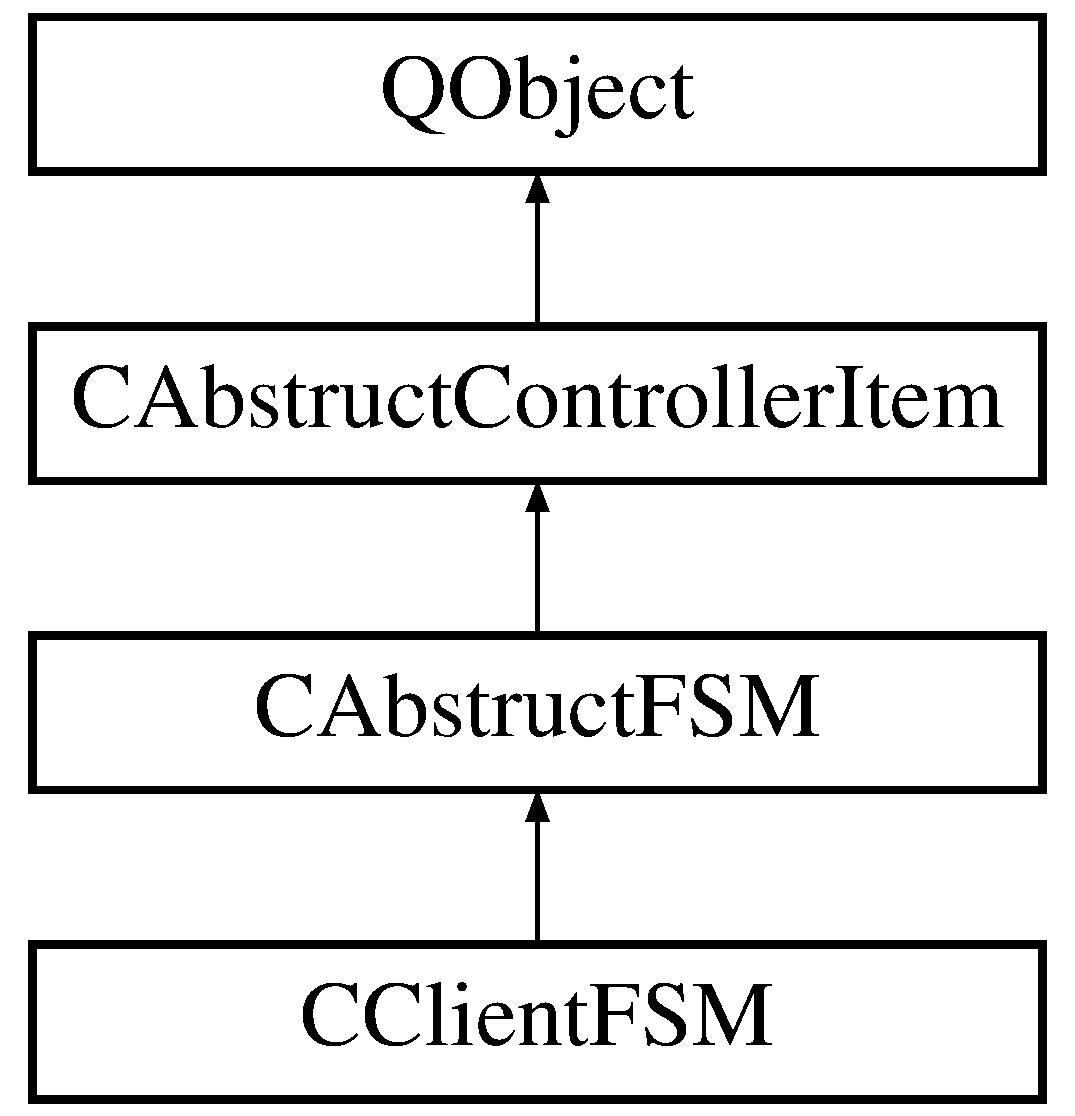
\includegraphics[height=4.000000cm]{class_c_client_f_s_m}
\end{center}
\end{figure}
\subsection*{Открытые члены}
\begin{DoxyCompactItemize}
\item 
\hyperlink{class_c_client_f_s_m_ad5cde8ac83f83aa722a1739bdf46a453}{C\+Client\+F\+SM} (Q\+Object $\ast$parent=0)
\item 
virtual \hyperlink{class_c_client_f_s_m_acd28280c438e234e05340ddb46472c2d}{$\sim$\+C\+Client\+F\+SM} ()
\end{DoxyCompactItemize}
\subsection*{Защищенные члены}
\begin{DoxyCompactItemize}
\item 
void \hyperlink{class_c_client_f_s_m_aaf6b857e9a5d2b2f55b71212e74fd4cb}{init\+Connections} ()
\begin{DoxyCompactList}\small\item\em Чисто виртуальный метод необходим для инициализации сигналов и слотов d классах наследниках. \end{DoxyCompactList}\end{DoxyCompactItemize}
\subsection*{Дополнительные унаследованные члены}


\subsection{Подробное описание}


См. определение в файле cclientfsm.\+h строка 7



\subsection{Конструктор(ы)}
\hypertarget{class_c_client_f_s_m_ad5cde8ac83f83aa722a1739bdf46a453}{}\label{class_c_client_f_s_m_ad5cde8ac83f83aa722a1739bdf46a453} 
\index{C\+Client\+F\+SM@{C\+Client\+F\+SM}!C\+Client\+F\+SM@{C\+Client\+F\+SM}}
\index{C\+Client\+F\+SM@{C\+Client\+F\+SM}!C\+Client\+F\+SM@{C\+Client\+F\+SM}}
\subsubsection{\texorpdfstring{C\+Client\+F\+S\+M()}{CClientFSM()}}
{\footnotesize\ttfamily C\+Client\+F\+S\+M\+::\+C\+Client\+F\+SM (\begin{DoxyParamCaption}\item[{Q\+Object $\ast$}]{parent = {\ttfamily 0} }\end{DoxyParamCaption})\hspace{0.3cm}{\ttfamily [explicit]}}



См. определение в файле cclientfsm.\+cpp строка 3



Перекрестные ссылки init\+Connections().


\begin{DoxyCode}
3                                      :
4     \hyperlink{class_c_abstruct_f_s_m_a54037c986f6b437c50d5e8ba42063330}{CAbstructFSM}(parent)
5 \{
6     \hyperlink{class_c_client_f_s_m_aaf6b857e9a5d2b2f55b71212e74fd4cb}{initConnections}();
7 \}
\end{DoxyCode}
\hypertarget{class_c_client_f_s_m_acd28280c438e234e05340ddb46472c2d}{}\label{class_c_client_f_s_m_acd28280c438e234e05340ddb46472c2d} 
\index{C\+Client\+F\+SM@{C\+Client\+F\+SM}!````~C\+Client\+F\+SM@{$\sim$\+C\+Client\+F\+SM}}
\index{````~C\+Client\+F\+SM@{$\sim$\+C\+Client\+F\+SM}!C\+Client\+F\+SM@{C\+Client\+F\+SM}}
\subsubsection{\texorpdfstring{$\sim$\+C\+Client\+F\+S\+M()}{~CClientFSM()}}
{\footnotesize\ttfamily C\+Client\+F\+S\+M\+::$\sim$\+C\+Client\+F\+SM (\begin{DoxyParamCaption}{ }\end{DoxyParamCaption})\hspace{0.3cm}{\ttfamily [virtual]}}



См. определение в файле cclientfsm.\+cpp строка 9


\begin{DoxyCode}
10 \{
11 
12 \}
\end{DoxyCode}


\subsection{Методы}
\hypertarget{class_c_client_f_s_m_aaf6b857e9a5d2b2f55b71212e74fd4cb}{}\label{class_c_client_f_s_m_aaf6b857e9a5d2b2f55b71212e74fd4cb} 
\index{C\+Client\+F\+SM@{C\+Client\+F\+SM}!init\+Connections@{init\+Connections}}
\index{init\+Connections@{init\+Connections}!C\+Client\+F\+SM@{C\+Client\+F\+SM}}
\subsubsection{\texorpdfstring{init\+Connections()}{initConnections()}}
{\footnotesize\ttfamily void C\+Client\+F\+S\+M\+::init\+Connections (\begin{DoxyParamCaption}{ }\end{DoxyParamCaption})\hspace{0.3cm}{\ttfamily [protected]}, {\ttfamily [virtual]}}



Чисто виртуальный метод необходим для инициализации сигналов и слотов d классах наследниках. 



Замещает \hyperlink{class_c_abstruct_controller_item_a27c6889230a86cb0782e6d7596b883c1}{C\+Abstruct\+Controller\+Item}.



См. определение в файле cclientfsm.\+cpp строка 14



Используется в C\+Client\+F\+S\+M().


\begin{DoxyCode}
15 \{
16 
17 \}
\end{DoxyCode}


Объявления и описания членов классов находятся в файлах\+:\begin{DoxyCompactItemize}
\item 
Client/\hyperlink{cclientfsm_8h}{cclientfsm.\+h}\item 
Client/\hyperlink{cclientfsm_8cpp}{cclientfsm.\+cpp}\end{DoxyCompactItemize}

\hypertarget{class_c_client_i_o_network_manager}{}\section{Класс C\+Client\+I\+O\+Network\+Manager}
\label{class_c_client_i_o_network_manager}\index{C\+Client\+I\+O\+Network\+Manager@{C\+Client\+I\+O\+Network\+Manager}}


{\ttfamily \#include $<$cclientionetworkmanager.\+h$>$}

Граф наследования\+:C\+Client\+I\+O\+Network\+Manager\+:\begin{figure}[H]
\begin{center}
\leavevmode
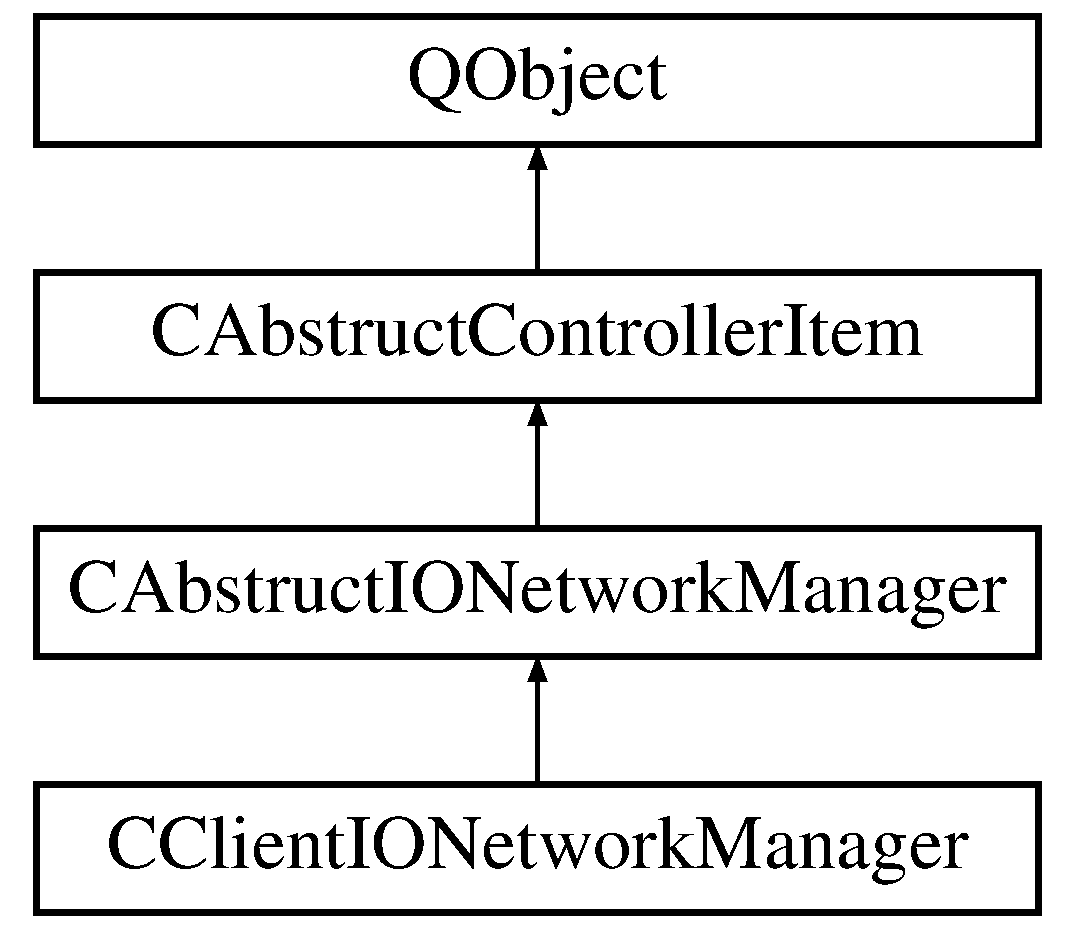
\includegraphics[height=4.000000cm]{class_c_client_i_o_network_manager}
\end{center}
\end{figure}
\subsection*{Открытые слоты}
\begin{DoxyCompactItemize}
\item 
void \hyperlink{class_c_client_i_o_network_manager_a1a4c3fd9405b85cb43e20b24d9db18e8}{error} (Q\+Abstract\+Socket\+::\+Socket\+Error)
\item 
void \hyperlink{class_c_client_i_o_network_manager_aaa7b77037603697d3bee7daed467b092}{connect\+To\+Host} ()
\end{DoxyCompactItemize}
\subsection*{Открытые члены}
\begin{DoxyCompactItemize}
\item 
\hyperlink{class_c_client_i_o_network_manager_af9f85db2c4a515cc974038086edc6b9f}{C\+Client\+I\+O\+Network\+Manager} (Q\+Tcp\+Socket $\ast$socket, Q\+Object $\ast$parent=0)
\item 
virtual \hyperlink{class_c_client_i_o_network_manager_aaaeddd1337640480b4eae0418cee6026}{$\sim$\+C\+Client\+I\+O\+Network\+Manager} ()
\end{DoxyCompactItemize}
\subsection*{Защищенные члены}
\begin{DoxyCompactItemize}
\item 
void \hyperlink{class_c_client_i_o_network_manager_aeb1564c209ae8b790cf799075cfa6a98}{init\+Connections} ()
\begin{DoxyCompactList}\small\item\em Чисто виртуальный метод необходим для инициализации сигналов и слотов d классах наследниках. \end{DoxyCompactList}\end{DoxyCompactItemize}
\subsection*{Дополнительные унаследованные члены}


\subsection{Подробное описание}


См. определение в файле cclientionetworkmanager.\+h строка 8



\subsection{Конструктор(ы)}
\hypertarget{class_c_client_i_o_network_manager_af9f85db2c4a515cc974038086edc6b9f}{}\label{class_c_client_i_o_network_manager_af9f85db2c4a515cc974038086edc6b9f} 
\index{C\+Client\+I\+O\+Network\+Manager@{C\+Client\+I\+O\+Network\+Manager}!C\+Client\+I\+O\+Network\+Manager@{C\+Client\+I\+O\+Network\+Manager}}
\index{C\+Client\+I\+O\+Network\+Manager@{C\+Client\+I\+O\+Network\+Manager}!C\+Client\+I\+O\+Network\+Manager@{C\+Client\+I\+O\+Network\+Manager}}
\subsubsection{\texorpdfstring{C\+Client\+I\+O\+Network\+Manager()}{CClientIONetworkManager()}}
{\footnotesize\ttfamily C\+Client\+I\+O\+Network\+Manager\+::\+C\+Client\+I\+O\+Network\+Manager (\begin{DoxyParamCaption}\item[{Q\+Tcp\+Socket $\ast$}]{socket,  }\item[{Q\+Object $\ast$}]{parent = {\ttfamily 0} }\end{DoxyParamCaption})\hspace{0.3cm}{\ttfamily [explicit]}}



См. определение в файле cclientionetworkmanager.\+cpp строка 3



Перекрестные ссылки init\+Connections().


\begin{DoxyCode}
3                                                                                    :
4     \hyperlink{class_c_abstruct_i_o_network_manager_a4ed201a3712ddf4ccd2135a0eb40fbf2}{CAbstructIONetworkManager}(socket, parent)
5 \{
6     \hyperlink{class_c_client_i_o_network_manager_aeb1564c209ae8b790cf799075cfa6a98}{initConnections}();
7 \}
\end{DoxyCode}
\hypertarget{class_c_client_i_o_network_manager_aaaeddd1337640480b4eae0418cee6026}{}\label{class_c_client_i_o_network_manager_aaaeddd1337640480b4eae0418cee6026} 
\index{C\+Client\+I\+O\+Network\+Manager@{C\+Client\+I\+O\+Network\+Manager}!````~C\+Client\+I\+O\+Network\+Manager@{$\sim$\+C\+Client\+I\+O\+Network\+Manager}}
\index{````~C\+Client\+I\+O\+Network\+Manager@{$\sim$\+C\+Client\+I\+O\+Network\+Manager}!C\+Client\+I\+O\+Network\+Manager@{C\+Client\+I\+O\+Network\+Manager}}
\subsubsection{\texorpdfstring{$\sim$\+C\+Client\+I\+O\+Network\+Manager()}{~CClientIONetworkManager()}}
{\footnotesize\ttfamily C\+Client\+I\+O\+Network\+Manager\+::$\sim$\+C\+Client\+I\+O\+Network\+Manager (\begin{DoxyParamCaption}{ }\end{DoxyParamCaption})\hspace{0.3cm}{\ttfamily [virtual]}}



См. определение в файле cclientionetworkmanager.\+cpp строка 9


\begin{DoxyCode}
10 \{
11 
12 \}
\end{DoxyCode}


\subsection{Методы}
\hypertarget{class_c_client_i_o_network_manager_aaa7b77037603697d3bee7daed467b092}{}\label{class_c_client_i_o_network_manager_aaa7b77037603697d3bee7daed467b092} 
\index{C\+Client\+I\+O\+Network\+Manager@{C\+Client\+I\+O\+Network\+Manager}!connect\+To\+Host@{connect\+To\+Host}}
\index{connect\+To\+Host@{connect\+To\+Host}!C\+Client\+I\+O\+Network\+Manager@{C\+Client\+I\+O\+Network\+Manager}}
\subsubsection{\texorpdfstring{connect\+To\+Host}{connectToHost}}
{\footnotesize\ttfamily void C\+Client\+I\+O\+Network\+Manager\+::connect\+To\+Host (\begin{DoxyParamCaption}{ }\end{DoxyParamCaption})\hspace{0.3cm}{\ttfamily [slot]}}



См. определение в файле cclientionetworkmanager.\+cpp строка 19



Перекрестные ссылки C\+Abstruct\+I\+O\+Network\+Manager\+::get\+Socket().


\begin{DoxyCode}
20 \{
21     \hyperlink{class_c_abstruct_i_o_network_manager_a118a2c8254c149614cba51c42147c709}{getSocket}()->connectToHost(\textcolor{stringliteral}{"192.168.100.2"}, 52816);
22 \}
\end{DoxyCode}
\hypertarget{class_c_client_i_o_network_manager_a1a4c3fd9405b85cb43e20b24d9db18e8}{}\label{class_c_client_i_o_network_manager_a1a4c3fd9405b85cb43e20b24d9db18e8} 
\index{C\+Client\+I\+O\+Network\+Manager@{C\+Client\+I\+O\+Network\+Manager}!error@{error}}
\index{error@{error}!C\+Client\+I\+O\+Network\+Manager@{C\+Client\+I\+O\+Network\+Manager}}
\subsubsection{\texorpdfstring{error}{error}}
{\footnotesize\ttfamily void C\+Client\+I\+O\+Network\+Manager\+::error (\begin{DoxyParamCaption}\item[{Q\+Abstract\+Socket\+::\+Socket\+Error}]{ }\end{DoxyParamCaption})\hspace{0.3cm}{\ttfamily [slot]}}



См. определение в файле cclientionetworkmanager.\+cpp строка 14



Перекрестные ссылки C\+Abstruct\+I\+O\+Network\+Manager\+::get\+Socket() и C\+Abstruct\+Controller\+Item\+::send\+Data().



Используется в init\+Connections().


\begin{DoxyCode}
15 \{
16     emit \hyperlink{class_c_abstruct_controller_item_a7cf2bebc87a7d0b660318e946a176eb9}{sendData}(\textcolor{keyword}{new} QString(\hyperlink{class_c_abstruct_i_o_network_manager_a118a2c8254c149614cba51c42147c709}{getSocket}()->errorString()));
17 \}
\end{DoxyCode}
\hypertarget{class_c_client_i_o_network_manager_aeb1564c209ae8b790cf799075cfa6a98}{}\label{class_c_client_i_o_network_manager_aeb1564c209ae8b790cf799075cfa6a98} 
\index{C\+Client\+I\+O\+Network\+Manager@{C\+Client\+I\+O\+Network\+Manager}!init\+Connections@{init\+Connections}}
\index{init\+Connections@{init\+Connections}!C\+Client\+I\+O\+Network\+Manager@{C\+Client\+I\+O\+Network\+Manager}}
\subsubsection{\texorpdfstring{init\+Connections()}{initConnections()}}
{\footnotesize\ttfamily void C\+Client\+I\+O\+Network\+Manager\+::init\+Connections (\begin{DoxyParamCaption}{ }\end{DoxyParamCaption})\hspace{0.3cm}{\ttfamily [protected]}, {\ttfamily [virtual]}}



Чисто виртуальный метод необходим для инициализации сигналов и слотов d классах наследниках. 



Замещает \hyperlink{class_c_abstruct_controller_item_a27c6889230a86cb0782e6d7596b883c1}{C\+Abstruct\+Controller\+Item}.



См. определение в файле cclientionetworkmanager.\+cpp строка 24



Перекрестные ссылки error() и C\+Abstruct\+I\+O\+Network\+Manager\+::get\+Socket().



Используется в C\+Client\+I\+O\+Network\+Manager().


\begin{DoxyCode}
25 \{
26     connect(this->\hyperlink{class_c_abstruct_i_o_network_manager_a118a2c8254c149614cba51c42147c709}{getSocket}(), SIGNAL(\hyperlink{class_c_client_i_o_network_manager_a1a4c3fd9405b85cb43e20b24d9db18e8}{error}(QAbstractSocket::SocketError)), \textcolor{keyword}{this}, SLOT(
      \hyperlink{class_c_client_i_o_network_manager_a1a4c3fd9405b85cb43e20b24d9db18e8}{error}(QAbstractSocket::SocketError)));
27 \}
\end{DoxyCode}


Объявления и описания членов классов находятся в файлах\+:\begin{DoxyCompactItemize}
\item 
Client/\hyperlink{cclientionetworkmanager_8h}{cclientionetworkmanager.\+h}\item 
Client/\hyperlink{cclientionetworkmanager_8cpp}{cclientionetworkmanager.\+cpp}\end{DoxyCompactItemize}

\hypertarget{class_c_server}{}\section{Класс C\+Server}
\label{class_c_server}\index{C\+Server@{C\+Server}}


Сервер  




{\ttfamily \#include $<$cserver.\+h$>$}

Граф наследования\+:C\+Server\+:\begin{figure}[H]
\begin{center}
\leavevmode
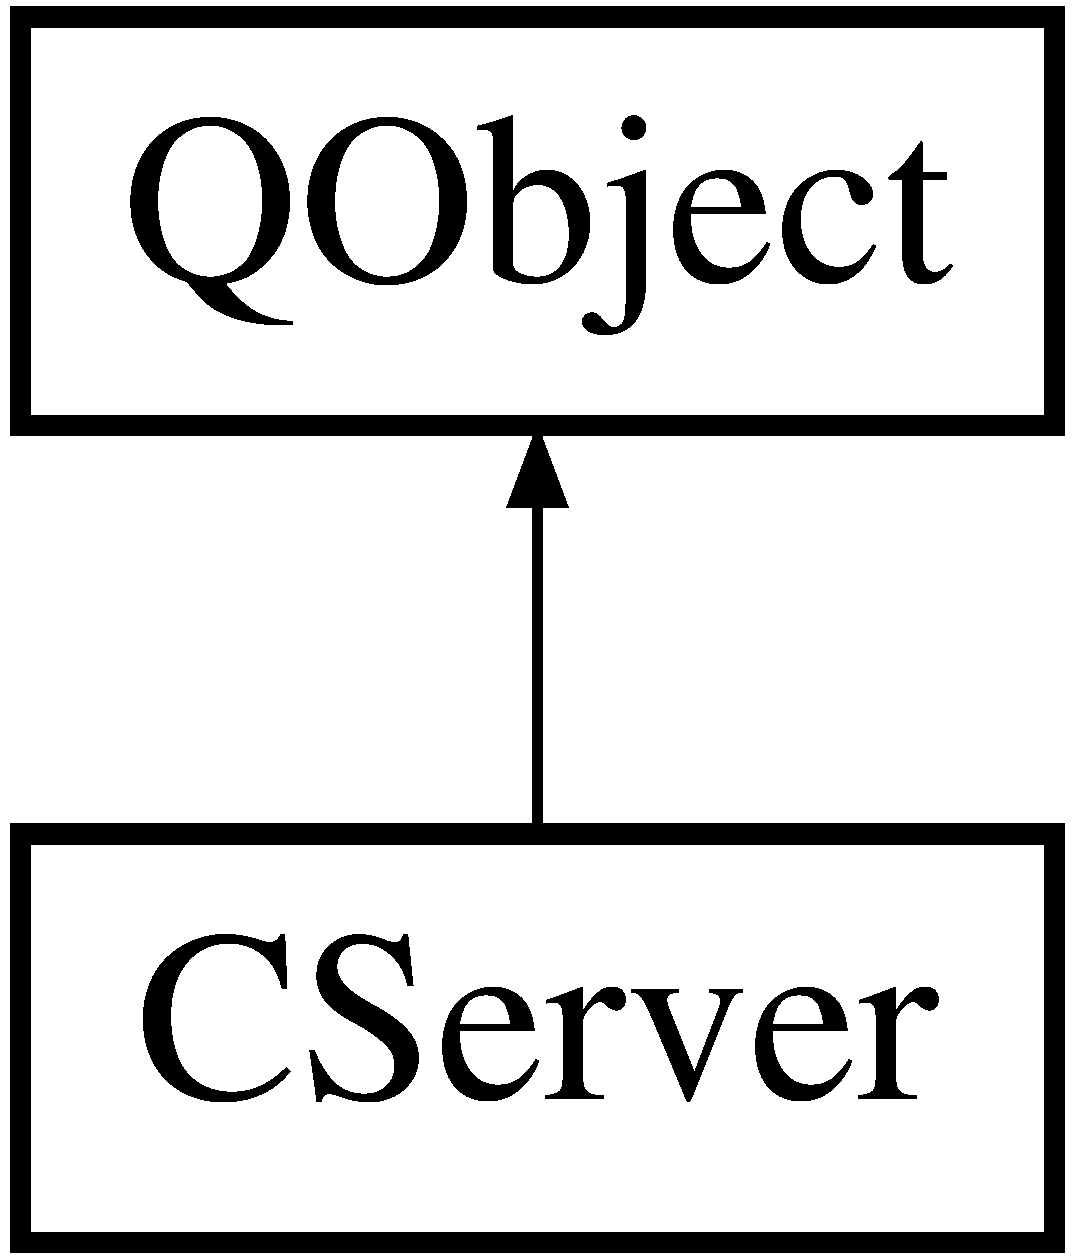
\includegraphics[height=2.000000cm]{class_c_server}
\end{center}
\end{figure}
\subsection*{Открытые слоты}
\begin{DoxyCompactItemize}
\item 
\hypertarget{class_c_server_a4e5b127e1eb4342a130018d9ff921735}{}\label{class_c_server_a4e5b127e1eb4342a130018d9ff921735} 
void {\bfseries new\+Connection} ()
\item 
\hypertarget{class_c_server_adbc93cef317eac86a09a0b7067c96cc1}{}\label{class_c_server_adbc93cef317eac86a09a0b7067c96cc1} 
void {\bfseries start\+Server} ()
\end{DoxyCompactItemize}
\subsection*{Открытые члены}
\begin{DoxyCompactItemize}
\item 
\hypertarget{class_c_server_a743d64a8f7c949de3de873735f726fcf}{}\label{class_c_server_a743d64a8f7c949de3de873735f726fcf} 
{\bfseries C\+Server} (Q\+Object $\ast$parent=0)
\item 
\hypertarget{class_c_server_a32c8f33336a76b36c2653553b970e76c}{}\label{class_c_server_a32c8f33336a76b36c2653553b970e76c} 
void {\bfseries init\+Connections} ()
\item 
\hypertarget{class_c_server_a3ad6eca8c26fc7852aaf1c626c84e220}{}\label{class_c_server_a3ad6eca8c26fc7852aaf1c626c84e220} 
Q\+Tcp\+Server $\ast$ {\bfseries get\+Server} () const
\end{DoxyCompactItemize}


\subsection{Подробное описание}
Сервер 

Объявления и описания членов классов находятся в файлах\+:\begin{DoxyCompactItemize}
\item 
cserver.\+h\item 
cserver.\+cpp\end{DoxyCompactItemize}

\hypertarget{class_c_server_controller}{}\section{Класс C\+Server\+Controller}
\label{class_c_server_controller}\index{C\+Server\+Controller@{C\+Server\+Controller}}
Граф наследования\+:C\+Server\+Controller\+:\begin{figure}[H]
\begin{center}
\leavevmode
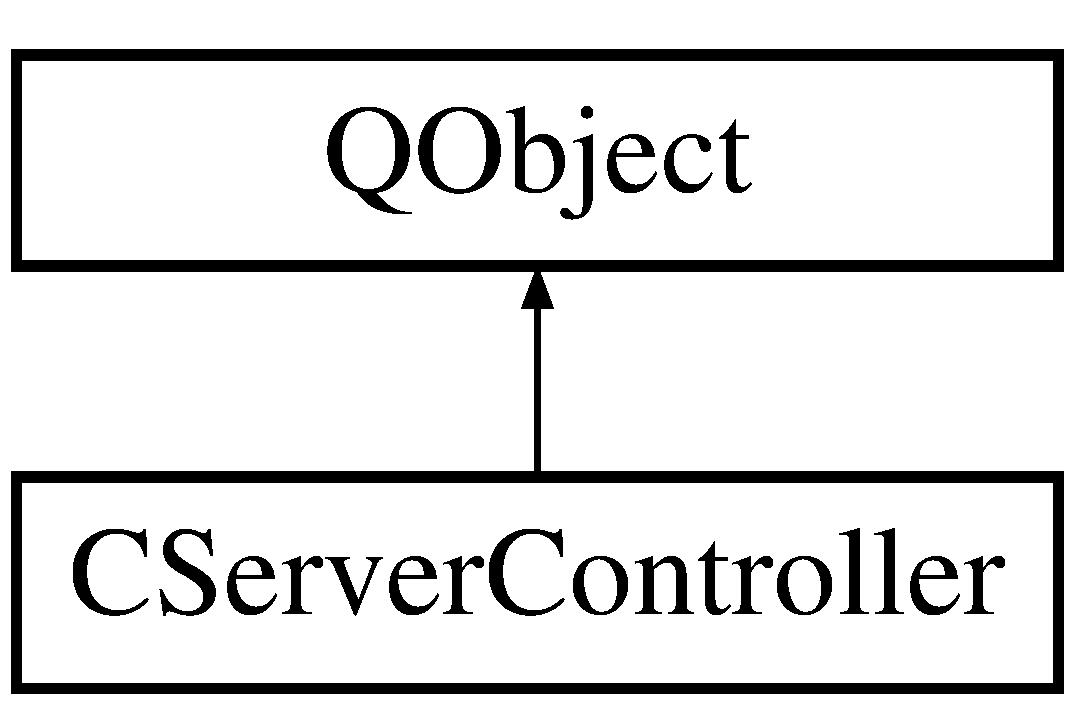
\includegraphics[height=2.000000cm]{class_c_server_controller}
\end{center}
\end{figure}
\subsection*{Сигналы}
\begin{DoxyCompactItemize}
\item 
\hypertarget{class_c_server_controller_a49ac8bb325430fc9112056d862c5c117}{}\label{class_c_server_controller_a49ac8bb325430fc9112056d862c5c117} 
void {\bfseries finish\+Work} ()
\end{DoxyCompactItemize}
\subsection*{Открытые члены}
\begin{DoxyCompactItemize}
\item 
\hypertarget{class_c_server_controller_ac7fa78891be114aa9ae1985541d5a766}{}\label{class_c_server_controller_ac7fa78891be114aa9ae1985541d5a766} 
{\bfseries C\+Server\+Controller} (Q\+Tcp\+Socket $\ast$socket, Q\+Object $\ast$parent=0)
\item 
\hypertarget{class_c_server_controller_a9934f4eb54e1e1debd1aa6fd5e036012}{}\label{class_c_server_controller_a9934f4eb54e1e1debd1aa6fd5e036012} 
\hyperlink{class_c_server_i_o_network_manager}{C\+Server\+I\+O\+Network\+Manager} $\ast$ {\bfseries get\+I\+O\+Network\+Manager} () const
\item 
\hypertarget{class_c_server_controller_ade77d98a3358e5b1914ebbffa7d810ce}{}\label{class_c_server_controller_ade77d98a3358e5b1914ebbffa7d810ce} 
\hyperlink{class_c_server_f_s_m}{C\+Server\+F\+SM} $\ast$ {\bfseries get\+F\+SM} () const
\item 
\hypertarget{class_c_server_controller_a2dc0dbf4a5ee9356f10b2156ad2ce712}{}\label{class_c_server_controller_a2dc0dbf4a5ee9356f10b2156ad2ce712} 
\hyperlink{class_c_server_d_b_manager}{C\+Server\+D\+B\+Manager} $\ast$ {\bfseries get\+D\+B\+Manager} () const
\item 
\hypertarget{class_c_server_controller_aeccfde1d541a9f57f8276cc6a24aea12}{}\label{class_c_server_controller_aeccfde1d541a9f57f8276cc6a24aea12} 
void {\bfseries init\+Connections} () const
\end{DoxyCompactItemize}


Объявления и описания членов классов находятся в файлах\+:\begin{DoxyCompactItemize}
\item 
cservercontroller.\+h\item 
cservercontroller.\+cpp\end{DoxyCompactItemize}

\hypertarget{class_c_server_d_b_manager}{}\section{Класс C\+Server\+D\+B\+Manager}
\label{class_c_server_d_b_manager}\index{C\+Server\+D\+B\+Manager@{C\+Server\+D\+B\+Manager}}


Класс работы с базой данных на сервере  




{\ttfamily \#include $<$cserverdbmanager.\+h$>$}

Граф наследования\+:C\+Server\+D\+B\+Manager\+:\begin{figure}[H]
\begin{center}
\leavevmode
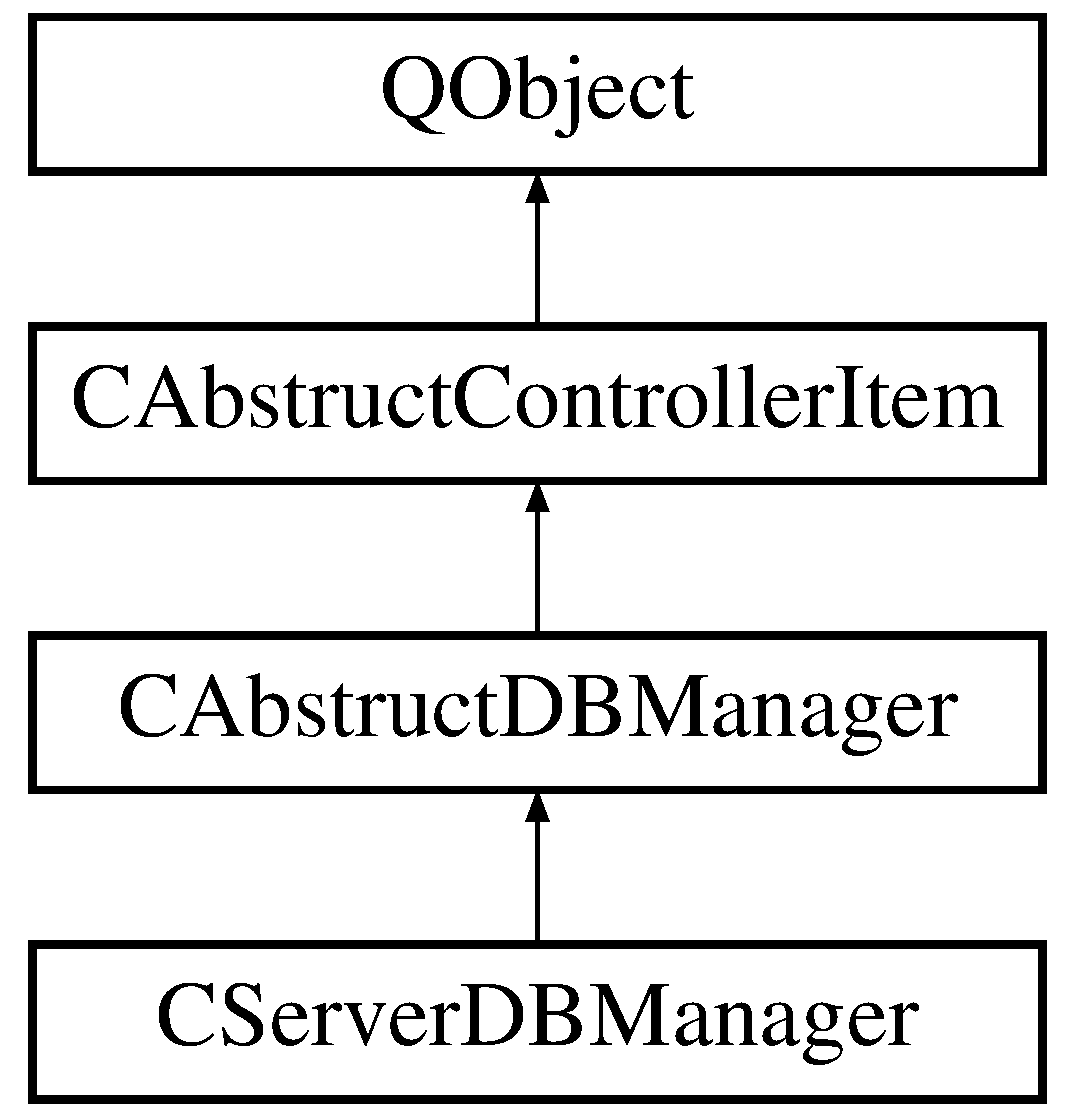
\includegraphics[height=4.000000cm]{class_c_server_d_b_manager}
\end{center}
\end{figure}
\subsection*{Открытые члены}
\begin{DoxyCompactItemize}
\item 
\hyperlink{class_c_server_d_b_manager_af2bf11fcced1aad0ccd34a3d16c45a03}{C\+Server\+D\+B\+Manager} (Q\+Object $\ast$parent=0)
\begin{DoxyCompactList}\small\item\em Конструктор. \end{DoxyCompactList}\item 
\hyperlink{class_c_server_d_b_manager_a78afc3d1890662a9bcbb3d184ac71141}{$\sim$\+C\+Server\+D\+B\+Manager} ()
\begin{DoxyCompactList}\small\item\em Деструктор. \end{DoxyCompactList}\end{DoxyCompactItemize}
\subsection*{Защищенные члены}
\begin{DoxyCompactItemize}
\item 
void \hyperlink{class_c_server_d_b_manager_a6dcd2f88c0845cc79a47bac2ab9e9235}{init\+Connections} ()
\begin{DoxyCompactList}\small\item\em Метод соединения сигналов и слотов. \end{DoxyCompactList}\end{DoxyCompactItemize}
\subsection*{Дополнительные унаследованные члены}


\subsection{Подробное описание}
Класс работы с базой данных на сервере 

См. определение в файле cserverdbmanager.\+h строка 10



\subsection{Конструктор(ы)}
\hypertarget{class_c_server_d_b_manager_af2bf11fcced1aad0ccd34a3d16c45a03}{}\label{class_c_server_d_b_manager_af2bf11fcced1aad0ccd34a3d16c45a03} 
\index{C\+Server\+D\+B\+Manager@{C\+Server\+D\+B\+Manager}!C\+Server\+D\+B\+Manager@{C\+Server\+D\+B\+Manager}}
\index{C\+Server\+D\+B\+Manager@{C\+Server\+D\+B\+Manager}!C\+Server\+D\+B\+Manager@{C\+Server\+D\+B\+Manager}}
\subsubsection{\texorpdfstring{C\+Server\+D\+B\+Manager()}{CServerDBManager()}}
{\footnotesize\ttfamily C\+Server\+D\+B\+Manager\+::\+C\+Server\+D\+B\+Manager (\begin{DoxyParamCaption}\item[{Q\+Object $\ast$}]{parent = {\ttfamily 0} }\end{DoxyParamCaption})}



Конструктор. 


\begin{DoxyParams}[1]{Аргументы}
\mbox{\tt in}  & {\em parent} & Указатель на объект верхнего уровня иерархии объектов.\\
\hline
\end{DoxyParams}
В конструкторе вызывается метод \hyperlink{class_c_server_d_b_manager_a6dcd2f88c0845cc79a47bac2ab9e9235}{init\+Connections()} для соединения сигналов и слотов. 

См. определение в файле cserverdbmanager.\+cpp строка 9



Перекрестные ссылки init\+Connections().


\begin{DoxyCode}
9                                                   :
10     \hyperlink{class_c_abstruct_d_b_manager_a53c2018cfa7a1a24bacd747967509bd7}{CAbstructDBManager}(parent)
11 \{
12     \hyperlink{class_c_server_d_b_manager_a6dcd2f88c0845cc79a47bac2ab9e9235}{initConnections}();
13 \}
\end{DoxyCode}
\hypertarget{class_c_server_d_b_manager_a78afc3d1890662a9bcbb3d184ac71141}{}\label{class_c_server_d_b_manager_a78afc3d1890662a9bcbb3d184ac71141} 
\index{C\+Server\+D\+B\+Manager@{C\+Server\+D\+B\+Manager}!````~C\+Server\+D\+B\+Manager@{$\sim$\+C\+Server\+D\+B\+Manager}}
\index{````~C\+Server\+D\+B\+Manager@{$\sim$\+C\+Server\+D\+B\+Manager}!C\+Server\+D\+B\+Manager@{C\+Server\+D\+B\+Manager}}
\subsubsection{\texorpdfstring{$\sim$\+C\+Server\+D\+B\+Manager()}{~CServerDBManager()}}
{\footnotesize\ttfamily C\+Server\+D\+B\+Manager\+::$\sim$\+C\+Server\+D\+B\+Manager (\begin{DoxyParamCaption}{ }\end{DoxyParamCaption})}



Деструктор. 



См. определение в файле cserverdbmanager.\+cpp строка 18


\begin{DoxyCode}
19 \{
20     qDebug() << \textcolor{stringliteral}{"CServerDBManager: destructor "} << \textcolor{keyword}{this};
21 \}
\end{DoxyCode}


\subsection{Методы}
\hypertarget{class_c_server_d_b_manager_a6dcd2f88c0845cc79a47bac2ab9e9235}{}\label{class_c_server_d_b_manager_a6dcd2f88c0845cc79a47bac2ab9e9235} 
\index{C\+Server\+D\+B\+Manager@{C\+Server\+D\+B\+Manager}!init\+Connections@{init\+Connections}}
\index{init\+Connections@{init\+Connections}!C\+Server\+D\+B\+Manager@{C\+Server\+D\+B\+Manager}}
\subsubsection{\texorpdfstring{init\+Connections()}{initConnections()}}
{\footnotesize\ttfamily void C\+Server\+D\+B\+Manager\+::init\+Connections (\begin{DoxyParamCaption}{ }\end{DoxyParamCaption})\hspace{0.3cm}{\ttfamily [protected]}, {\ttfamily [virtual]}}



Метод соединения сигналов и слотов. 



Переопределяет метод предка \hyperlink{class_c_abstruct_d_b_manager_ad450c557df6d9a7dfcc4a37082f35659}{C\+Abstruct\+D\+B\+Manager}.



См. определение в файле cserverdbmanager.\+cpp строка 26



Используется в C\+Server\+D\+B\+Manager().


\begin{DoxyCode}
27 \{
28 
29 \}
\end{DoxyCode}


Объявления и описания членов классов находятся в файлах\+:\begin{DoxyCompactItemize}
\item 
Server/\hyperlink{cserverdbmanager_8h}{cserverdbmanager.\+h}\item 
Server/\hyperlink{cserverdbmanager_8cpp}{cserverdbmanager.\+cpp}\end{DoxyCompactItemize}

\hypertarget{class_c_server_f_s_m}{}\section{Класс C\+Server\+F\+SM}
\label{class_c_server_f_s_m}\index{C\+Server\+F\+SM@{C\+Server\+F\+SM}}


Класс работы с конечным автоматом сервера.  




{\ttfamily \#include $<$cserverfsm.\+h$>$}

Граф наследования\+:C\+Server\+F\+SM\+:\begin{figure}[H]
\begin{center}
\leavevmode
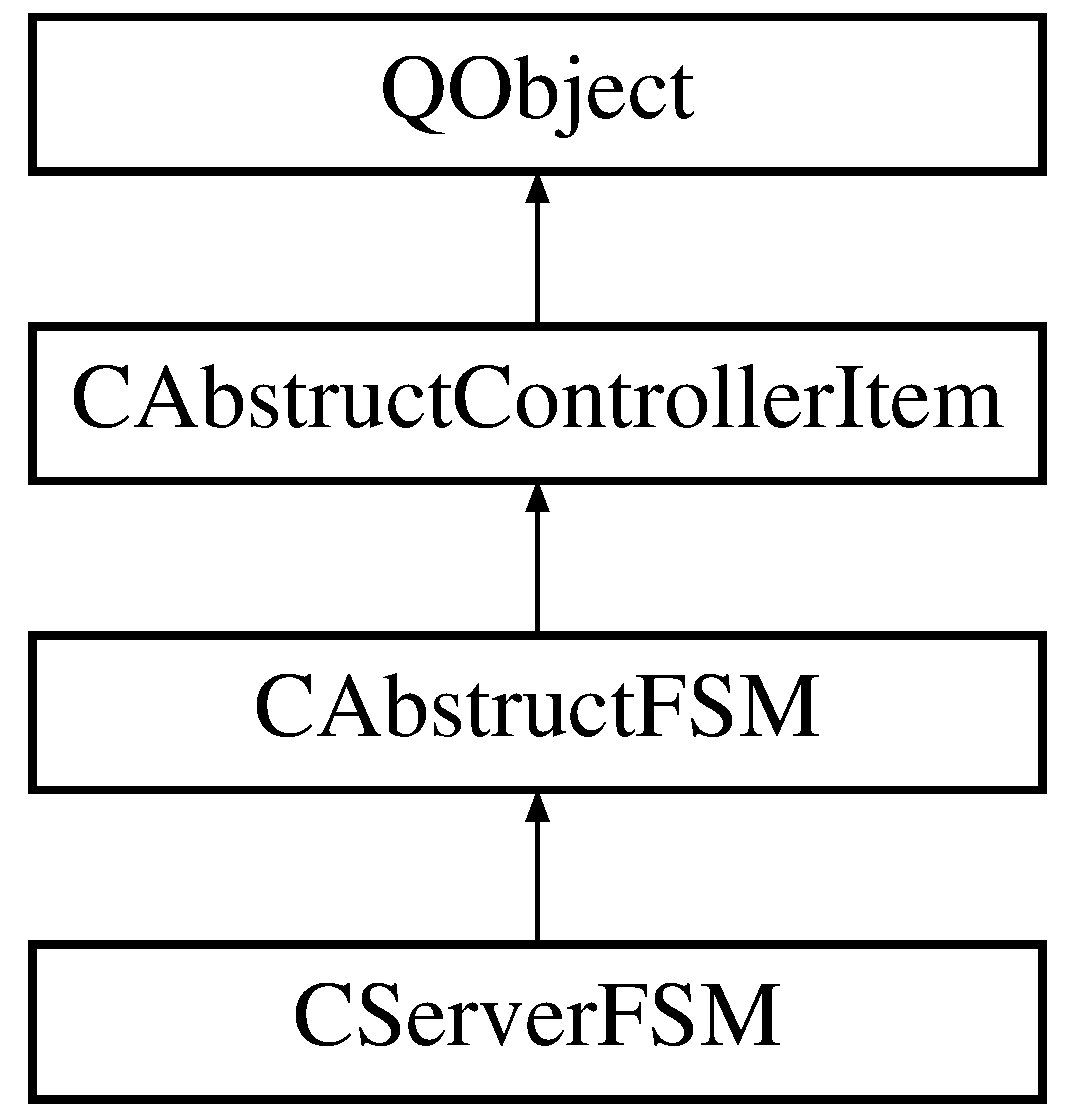
\includegraphics[height=4.000000cm]{class_c_server_f_s_m}
\end{center}
\end{figure}
\subsection*{Открытые члены}
\begin{DoxyCompactItemize}
\item 
\hyperlink{class_c_server_f_s_m_a6d2328de2b1e2725e4a569e146b077f3}{C\+Server\+F\+SM} (Q\+Object $\ast$parent=0)
\begin{DoxyCompactList}\small\item\em Конструктор. \end{DoxyCompactList}\item 
\hyperlink{class_c_server_f_s_m_a33dcbbf4680177c3f5769171f9516e8c}{$\sim$\+C\+Server\+F\+SM} ()
\begin{DoxyCompactList}\small\item\em Деструктор. \end{DoxyCompactList}\end{DoxyCompactItemize}
\subsection*{Защищенные члены}
\begin{DoxyCompactItemize}
\item 
void \hyperlink{class_c_server_f_s_m_ae0e6a994505c26e60b718af9989bea77}{init\+Connections} ()
\begin{DoxyCompactList}\small\item\em Метод инициализации соединений сигналов и слотов. \end{DoxyCompactList}\end{DoxyCompactItemize}
\subsection*{Дополнительные унаследованные члены}


\subsection{Подробное описание}
Класс работы с конечным автоматом сервера. 

См. определение в файле cserverfsm.\+h строка 10



\subsection{Конструктор(ы)}
\hypertarget{class_c_server_f_s_m_a6d2328de2b1e2725e4a569e146b077f3}{}\label{class_c_server_f_s_m_a6d2328de2b1e2725e4a569e146b077f3} 
\index{C\+Server\+F\+SM@{C\+Server\+F\+SM}!C\+Server\+F\+SM@{C\+Server\+F\+SM}}
\index{C\+Server\+F\+SM@{C\+Server\+F\+SM}!C\+Server\+F\+SM@{C\+Server\+F\+SM}}
\subsubsection{\texorpdfstring{C\+Server\+F\+S\+M()}{CServerFSM()}}
{\footnotesize\ttfamily C\+Server\+F\+S\+M\+::\+C\+Server\+F\+SM (\begin{DoxyParamCaption}\item[{Q\+Object $\ast$}]{parent = {\ttfamily 0} }\end{DoxyParamCaption})}



Конструктор. 


\begin{DoxyParams}[1]{Аргументы}
\mbox{\tt in}  & {\em parent} & Указатель на объект верхнего уровня иерархии объектов.\\
\hline
\end{DoxyParams}
В конструкторе вызывается метод \hyperlink{class_c_server_f_s_m_ae0e6a994505c26e60b718af9989bea77}{init\+Connections()} инициализации соединений сигналов и слотов. 

См. определение в файле cserverfsm.\+cpp строка 9



Перекрестные ссылки init\+Connections().


\begin{DoxyCode}
9                                       :
10     \hyperlink{class_c_abstruct_f_s_m_a54037c986f6b437c50d5e8ba42063330}{CAbstructFSM}(parent)
11 \{
12     \hyperlink{class_c_server_f_s_m_ae0e6a994505c26e60b718af9989bea77}{initConnections}();
13 \}
\end{DoxyCode}
\hypertarget{class_c_server_f_s_m_a33dcbbf4680177c3f5769171f9516e8c}{}\label{class_c_server_f_s_m_a33dcbbf4680177c3f5769171f9516e8c} 
\index{C\+Server\+F\+SM@{C\+Server\+F\+SM}!````~C\+Server\+F\+SM@{$\sim$\+C\+Server\+F\+SM}}
\index{````~C\+Server\+F\+SM@{$\sim$\+C\+Server\+F\+SM}!C\+Server\+F\+SM@{C\+Server\+F\+SM}}
\subsubsection{\texorpdfstring{$\sim$\+C\+Server\+F\+S\+M()}{~CServerFSM()}}
{\footnotesize\ttfamily C\+Server\+F\+S\+M\+::$\sim$\+C\+Server\+F\+SM (\begin{DoxyParamCaption}{ }\end{DoxyParamCaption})}



Деструктор. 



См. определение в файле cserverfsm.\+cpp строка 18


\begin{DoxyCode}
19 \{
20     qDebug() << \textcolor{stringliteral}{"CServerFSM: destructor "} << \textcolor{keyword}{this};
21 \}
\end{DoxyCode}


\subsection{Методы}
\hypertarget{class_c_server_f_s_m_ae0e6a994505c26e60b718af9989bea77}{}\label{class_c_server_f_s_m_ae0e6a994505c26e60b718af9989bea77} 
\index{C\+Server\+F\+SM@{C\+Server\+F\+SM}!init\+Connections@{init\+Connections}}
\index{init\+Connections@{init\+Connections}!C\+Server\+F\+SM@{C\+Server\+F\+SM}}
\subsubsection{\texorpdfstring{init\+Connections()}{initConnections()}}
{\footnotesize\ttfamily void C\+Server\+F\+S\+M\+::init\+Connections (\begin{DoxyParamCaption}{ }\end{DoxyParamCaption})\hspace{0.3cm}{\ttfamily [protected]}, {\ttfamily [virtual]}}



Метод инициализации соединений сигналов и слотов. 



Переопределяет метод предка \hyperlink{class_c_abstruct_f_s_m_a9d6f4659a08f3028f8c047243f8dcfc3}{C\+Abstruct\+F\+SM}.



См. определение в файле cserverfsm.\+cpp строка 26



Используется в C\+Server\+F\+S\+M().


\begin{DoxyCode}
27 \{
28 
29 \}
\end{DoxyCode}


Объявления и описания членов классов находятся в файлах\+:\begin{DoxyCompactItemize}
\item 
Server/\hyperlink{cserverfsm_8h}{cserverfsm.\+h}\item 
Server/\hyperlink{cserverfsm_8cpp}{cserverfsm.\+cpp}\end{DoxyCompactItemize}

\hypertarget{class_c_server_i_o_network_manager}{}\section{Класс C\+Server\+I\+O\+Network\+Manager}
\label{class_c_server_i_o_network_manager}\index{C\+Server\+I\+O\+Network\+Manager@{C\+Server\+I\+O\+Network\+Manager}}


Класс работы с сетью на сервере.  




{\ttfamily \#include $<$cserverionetworkmanager.\+h$>$}

Граф наследования\+:C\+Server\+I\+O\+Network\+Manager\+:\begin{figure}[H]
\begin{center}
\leavevmode
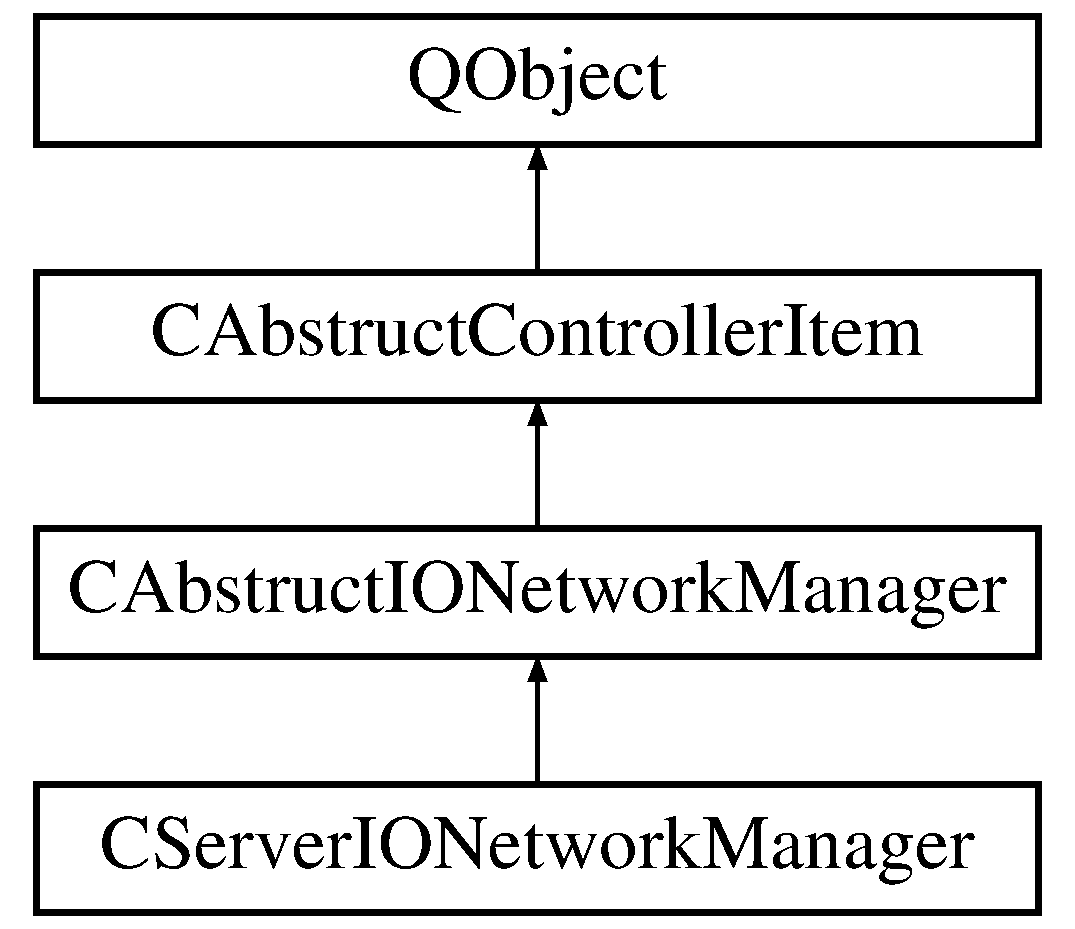
\includegraphics[height=4.000000cm]{class_c_server_i_o_network_manager}
\end{center}
\end{figure}
\subsection*{Открытые слоты}
\begin{DoxyCompactItemize}
\item 
void \hyperlink{class_c_server_i_o_network_manager_a27831f1d8f66c1e0d665c2ef52d262e4}{error\+Print} (Q\+Abstract\+Socket\+::\+Socket\+Error)
\begin{DoxyCompactList}\small\item\em Слот вывода в консоль ошибок работы сокета. \end{DoxyCompactList}\end{DoxyCompactItemize}
\subsection*{Открытые члены}
\begin{DoxyCompactItemize}
\item 
\hyperlink{class_c_server_i_o_network_manager_a89afb0912a02b5745aaad5ccea706304}{C\+Server\+I\+O\+Network\+Manager} (Q\+Tcp\+Socket $\ast$socket, Q\+Object $\ast$parent=0)
\begin{DoxyCompactList}\small\item\em Конструктор. \end{DoxyCompactList}\item 
\hyperlink{class_c_server_i_o_network_manager_a513fe280d83eab4b89054eac2fb27e0d}{$\sim$\+C\+Server\+I\+O\+Network\+Manager} ()
\begin{DoxyCompactList}\small\item\em Деструктор. \end{DoxyCompactList}\end{DoxyCompactItemize}
\subsection*{Защищенные члены}
\begin{DoxyCompactItemize}
\item 
void \hyperlink{class_c_server_i_o_network_manager_a17155570c51dc951db52d827f120c689}{init\+Connections} ()
\begin{DoxyCompactList}\small\item\em Метод инициализации сигналов и слотов. \end{DoxyCompactList}\end{DoxyCompactItemize}
\subsection*{Дополнительные унаследованные члены}


\subsection{Подробное описание}
Класс работы с сетью на сервере. 

См. определение в файле cserverionetworkmanager.\+h строка 10



\subsection{Конструктор(ы)}
\hypertarget{class_c_server_i_o_network_manager_a89afb0912a02b5745aaad5ccea706304}{}\label{class_c_server_i_o_network_manager_a89afb0912a02b5745aaad5ccea706304} 
\index{C\+Server\+I\+O\+Network\+Manager@{C\+Server\+I\+O\+Network\+Manager}!C\+Server\+I\+O\+Network\+Manager@{C\+Server\+I\+O\+Network\+Manager}}
\index{C\+Server\+I\+O\+Network\+Manager@{C\+Server\+I\+O\+Network\+Manager}!C\+Server\+I\+O\+Network\+Manager@{C\+Server\+I\+O\+Network\+Manager}}
\subsubsection{\texorpdfstring{C\+Server\+I\+O\+Network\+Manager()}{CServerIONetworkManager()}}
{\footnotesize\ttfamily C\+Server\+I\+O\+Network\+Manager\+::\+C\+Server\+I\+O\+Network\+Manager (\begin{DoxyParamCaption}\item[{Q\+Tcp\+Socket $\ast$}]{socket,  }\item[{Q\+Object $\ast$}]{parent = {\ttfamily 0} }\end{DoxyParamCaption})}



Конструктор. 


\begin{DoxyParams}[1]{Аргументы}
\mbox{\tt in}  & {\em socket} & Указатель на сокет подключенного к серверу клиента. \\
\hline
\mbox{\tt in}  & {\em parent} & Указатель на объект верхнего уровня в иерархии объектов.\\
\hline
\end{DoxyParams}
В конструкторе вызывается метод \hyperlink{class_c_server_i_o_network_manager_a17155570c51dc951db52d827f120c689}{init\+Connections()} инициализации соединений сигналов и слотов. 

См. определение в файле cserverionetworkmanager.\+cpp строка 11



Перекрестные ссылки init\+Connections().


\begin{DoxyCode}
11                                                                                     :
12     \hyperlink{class_c_abstruct_i_o_network_manager_a4ed201a3712ddf4ccd2135a0eb40fbf2}{CAbstructIONetworkManager}(socket, parent)
13 \{
14     \hyperlink{class_c_server_i_o_network_manager_a17155570c51dc951db52d827f120c689}{initConnections}();
15 \}
\end{DoxyCode}
\hypertarget{class_c_server_i_o_network_manager_a513fe280d83eab4b89054eac2fb27e0d}{}\label{class_c_server_i_o_network_manager_a513fe280d83eab4b89054eac2fb27e0d} 
\index{C\+Server\+I\+O\+Network\+Manager@{C\+Server\+I\+O\+Network\+Manager}!````~C\+Server\+I\+O\+Network\+Manager@{$\sim$\+C\+Server\+I\+O\+Network\+Manager}}
\index{````~C\+Server\+I\+O\+Network\+Manager@{$\sim$\+C\+Server\+I\+O\+Network\+Manager}!C\+Server\+I\+O\+Network\+Manager@{C\+Server\+I\+O\+Network\+Manager}}
\subsubsection{\texorpdfstring{$\sim$\+C\+Server\+I\+O\+Network\+Manager()}{~CServerIONetworkManager()}}
{\footnotesize\ttfamily C\+Server\+I\+O\+Network\+Manager\+::$\sim$\+C\+Server\+I\+O\+Network\+Manager (\begin{DoxyParamCaption}{ }\end{DoxyParamCaption})}



Деструктор. 



См. определение в файле cserverionetworkmanager.\+cpp строка 20


\begin{DoxyCode}
21 \{
22     qDebug() << \textcolor{stringliteral}{"CServerIONetworkManager: destructor "} << \textcolor{keyword}{this};
23 \}
\end{DoxyCode}


\subsection{Методы}
\hypertarget{class_c_server_i_o_network_manager_a27831f1d8f66c1e0d665c2ef52d262e4}{}\label{class_c_server_i_o_network_manager_a27831f1d8f66c1e0d665c2ef52d262e4} 
\index{C\+Server\+I\+O\+Network\+Manager@{C\+Server\+I\+O\+Network\+Manager}!error\+Print@{error\+Print}}
\index{error\+Print@{error\+Print}!C\+Server\+I\+O\+Network\+Manager@{C\+Server\+I\+O\+Network\+Manager}}
\subsubsection{\texorpdfstring{error\+Print}{errorPrint}}
{\footnotesize\ttfamily void C\+Server\+I\+O\+Network\+Manager\+::error\+Print (\begin{DoxyParamCaption}\item[{Q\+Abstract\+Socket\+::\+Socket\+Error}]{ }\end{DoxyParamCaption})\hspace{0.3cm}{\ttfamily [slot]}}



Слот вывода в консоль ошибок работы сокета. 



См. определение в файле cserverionetworkmanager.\+cpp строка 40



Перекрестные ссылки C\+Abstruct\+I\+O\+Network\+Manager\+::get\+Socket().



Используется в init\+Connections().


\begin{DoxyCode}
41 \{
42     qDebug() << \hyperlink{class_c_abstruct_i_o_network_manager_a118a2c8254c149614cba51c42147c709}{getSocket}()->errorString();
43 \}
\end{DoxyCode}
\hypertarget{class_c_server_i_o_network_manager_a17155570c51dc951db52d827f120c689}{}\label{class_c_server_i_o_network_manager_a17155570c51dc951db52d827f120c689} 
\index{C\+Server\+I\+O\+Network\+Manager@{C\+Server\+I\+O\+Network\+Manager}!init\+Connections@{init\+Connections}}
\index{init\+Connections@{init\+Connections}!C\+Server\+I\+O\+Network\+Manager@{C\+Server\+I\+O\+Network\+Manager}}
\subsubsection{\texorpdfstring{init\+Connections()}{initConnections()}}
{\footnotesize\ttfamily void C\+Server\+I\+O\+Network\+Manager\+::init\+Connections (\begin{DoxyParamCaption}{ }\end{DoxyParamCaption})\hspace{0.3cm}{\ttfamily [protected]}, {\ttfamily [virtual]}}



Метод инициализации сигналов и слотов. 

Сигнал socket\textquotesingle{}a \hyperlink{class_c_server_i_o_network_manager_a27831f1d8f66c1e0d665c2ef52d262e4}{error\+Print()} соединяется со слотом C\+Server\+I\+O\+Networ\+Manager\+::error\+Print(). Если сокет генерирует сигнал об ошибке, то слот объекта работы с сетью выводит ошибку с консоль.

Переопределяет метод предка \hyperlink{class_c_abstruct_i_o_network_manager_ac01bfefacfa37050c8d3a9317a38fbf5}{C\+Abstruct\+I\+O\+Network\+Manager}.



См. определение в файле cserverionetworkmanager.\+cpp строка 28



Перекрестные ссылки error\+Print() и C\+Abstruct\+I\+O\+Network\+Manager\+::get\+Socket().



Используется в C\+Server\+I\+O\+Network\+Manager().


\begin{DoxyCode}
29 \{
34     connect(\hyperlink{class_c_abstruct_i_o_network_manager_a118a2c8254c149614cba51c42147c709}{getSocket}(), SIGNAL(error(QAbstractSocket::SocketError)), SLOT(
      \hyperlink{class_c_server_i_o_network_manager_a27831f1d8f66c1e0d665c2ef52d262e4}{errorPrint}(QAbstractSocket::SocketError)));
35 \}
\end{DoxyCode}


Объявления и описания членов классов находятся в файлах\+:\begin{DoxyCompactItemize}
\item 
Server/\hyperlink{cserverionetworkmanager_8h}{cserverionetworkmanager.\+h}\item 
Server/\hyperlink{cserverionetworkmanager_8cpp}{cserverionetworkmanager.\+cpp}\end{DoxyCompactItemize}

\hypertarget{class_main_window}{}\section{Класс Main\+Window}
\label{class_main_window}\index{Main\+Window@{Main\+Window}}


{\ttfamily \#include $<$mainwindow.\+h$>$}

Граф наследования\+:Main\+Window\+:\begin{figure}[H]
\begin{center}
\leavevmode
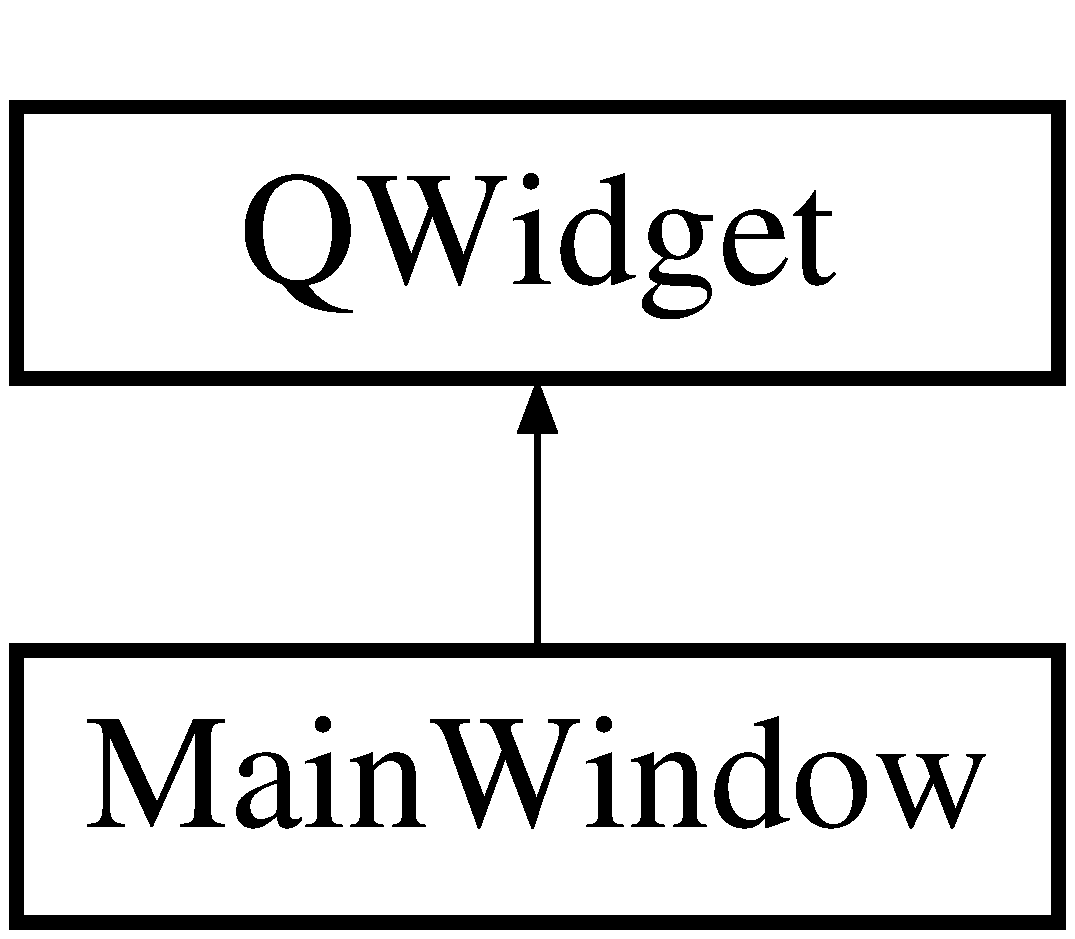
\includegraphics[height=2.000000cm]{class_main_window}
\end{center}
\end{figure}
\subsection*{Открытые члены}
\begin{DoxyCompactItemize}
\item 
\hyperlink{class_main_window_a8b244be8b7b7db1b08de2a2acb9409db}{Main\+Window} (Q\+Widget $\ast$parent=0)
\item 
\hyperlink{class_main_window_ae98d00a93bc118200eeef9f9bba1dba7}{$\sim$\+Main\+Window} ()
\item 
void \hyperlink{class_main_window_aecba599b372d9fdf89dfbc1f4a060019}{init\+Connections} ()
\end{DoxyCompactItemize}
\subsection*{Закрытые данные}
\begin{DoxyCompactItemize}
\item 
Q\+Label $\ast$ \hyperlink{class_main_window_a95477871d987adcaef8cfea7b87e27b0}{label1}
\item 
Q\+Label $\ast$ \hyperlink{class_main_window_ae83149c8748d57de45e882c51baef867}{label2}
\item 
Q\+Line\+Edit $\ast$ \hyperlink{class_main_window_af08619c735ace803854d9f3fc6fdf4d2}{line1}
\item 
Q\+Line\+Edit $\ast$ \hyperlink{class_main_window_a6bfac503123591b8bb31fd8e7dddd0c3}{line2}
\item 
Q\+Push\+Button $\ast$ \hyperlink{class_main_window_a96ee7d6a31dd131de9220930822f9da7}{button1}
\item 
Q\+Push\+Button $\ast$ \hyperlink{class_main_window_ad24e1c4eebdd74c9aadeea1f4c98414f}{button2}
\item 
Q\+Grid\+Layout $\ast$ \hyperlink{class_main_window_a152a77e5d13ba05ca3deb8cec9ab0365}{grid}
\item 
\hyperlink{class_c_client_controller}{C\+Client\+Controller} $\ast$ \hyperlink{class_main_window_af1f864005894311612c0b9174f82db8a}{controller}
\end{DoxyCompactItemize}


\subsection{Подробное описание}


См. определение в файле mainwindow.\+h строка 12



\subsection{Конструктор(ы)}
\hypertarget{class_main_window_a8b244be8b7b7db1b08de2a2acb9409db}{}\label{class_main_window_a8b244be8b7b7db1b08de2a2acb9409db} 
\index{Main\+Window@{Main\+Window}!Main\+Window@{Main\+Window}}
\index{Main\+Window@{Main\+Window}!Main\+Window@{Main\+Window}}
\subsubsection{\texorpdfstring{Main\+Window()}{MainWindow()}}
{\footnotesize\ttfamily Main\+Window\+::\+Main\+Window (\begin{DoxyParamCaption}\item[{Q\+Widget $\ast$}]{parent = {\ttfamily 0} }\end{DoxyParamCaption})}



См. определение в файле mainwindow.\+cpp строка 3



Перекрестные ссылки button1, button2, controller, grid, init\+Connections(), label1, label2, line1 и line2.


\begin{DoxyCode}
4     : QWidget(parent), \hyperlink{class_main_window_af1f864005894311612c0b9174f82db8a}{controller}(0)
5 \{
6     \hyperlink{class_main_window_af1f864005894311612c0b9174f82db8a}{controller} = \textcolor{keyword}{new} \hyperlink{class_c_client_controller}{CClientController}(\textcolor{keyword}{new} QTcpSocket(), \textcolor{keyword}{this});
7 
8     this->setWindowTitle(\textcolor{stringliteral}{"Authorization"});
9 
10     \hyperlink{class_main_window_a152a77e5d13ba05ca3deb8cec9ab0365}{grid} = \textcolor{keyword}{new} QGridLayout();
11     \hyperlink{class_main_window_a95477871d987adcaef8cfea7b87e27b0}{label1} = \textcolor{keyword}{new} QLabel(\textcolor{stringliteral}{"Login"});
12     \hyperlink{class_main_window_a95477871d987adcaef8cfea7b87e27b0}{label1}->setAlignment(Qt::AlignLeft);
13     \hyperlink{class_main_window_ae83149c8748d57de45e882c51baef867}{label2} = \textcolor{keyword}{new} QLabel(\textcolor{stringliteral}{"Password"});
14     \hyperlink{class_main_window_ae83149c8748d57de45e882c51baef867}{label2}->setAlignment(Qt::AlignLeft);
15     \hyperlink{class_main_window_af08619c735ace803854d9f3fc6fdf4d2}{line1} = \textcolor{keyword}{new} QLineEdit();
16     \hyperlink{class_main_window_af08619c735ace803854d9f3fc6fdf4d2}{line1}->setFixedWidth(100);
17     \hyperlink{class_main_window_a6bfac503123591b8bb31fd8e7dddd0c3}{line2} = \textcolor{keyword}{new} QLineEdit();
18     \hyperlink{class_main_window_a6bfac503123591b8bb31fd8e7dddd0c3}{line2}->setFixedWidth(100);
19     \hyperlink{class_main_window_a96ee7d6a31dd131de9220930822f9da7}{button1} = \textcolor{keyword}{new} QPushButton(\textcolor{stringliteral}{"Enter"});
20     \hyperlink{class_main_window_ad24e1c4eebdd74c9aadeea1f4c98414f}{button2} = \textcolor{keyword}{new} QPushButton(\textcolor{stringliteral}{"Registration"});
21 
22     \hyperlink{class_main_window_a152a77e5d13ba05ca3deb8cec9ab0365}{grid}->addWidget(\hyperlink{class_main_window_a95477871d987adcaef8cfea7b87e27b0}{label1}, 0, 0, 1, 1);
23     \hyperlink{class_main_window_a152a77e5d13ba05ca3deb8cec9ab0365}{grid}->addWidget(\hyperlink{class_main_window_af08619c735ace803854d9f3fc6fdf4d2}{line1}, 0, 1, 1, 1);
24     \hyperlink{class_main_window_a152a77e5d13ba05ca3deb8cec9ab0365}{grid}->addWidget(\hyperlink{class_main_window_ae83149c8748d57de45e882c51baef867}{label2}, 1, 0, 1, 1);
25     \hyperlink{class_main_window_a152a77e5d13ba05ca3deb8cec9ab0365}{grid}->addWidget(\hyperlink{class_main_window_a6bfac503123591b8bb31fd8e7dddd0c3}{line2}, 1, 1, 1, 1);
26     \hyperlink{class_main_window_a152a77e5d13ba05ca3deb8cec9ab0365}{grid}->addWidget(\hyperlink{class_main_window_a96ee7d6a31dd131de9220930822f9da7}{button1}, 2, 0, 1, 2);
27     \hyperlink{class_main_window_a152a77e5d13ba05ca3deb8cec9ab0365}{grid}->addWidget(\hyperlink{class_main_window_ad24e1c4eebdd74c9aadeea1f4c98414f}{button2}, 3, 0, 1, 2);
28 
29     setLayout(\hyperlink{class_main_window_a152a77e5d13ba05ca3deb8cec9ab0365}{grid});
30 
31     setFixedSize(sizeHint());
32 
33     \hyperlink{class_main_window_aecba599b372d9fdf89dfbc1f4a060019}{initConnections}();
34 
35 \}
\end{DoxyCode}
\hypertarget{class_main_window_ae98d00a93bc118200eeef9f9bba1dba7}{}\label{class_main_window_ae98d00a93bc118200eeef9f9bba1dba7} 
\index{Main\+Window@{Main\+Window}!````~Main\+Window@{$\sim$\+Main\+Window}}
\index{````~Main\+Window@{$\sim$\+Main\+Window}!Main\+Window@{Main\+Window}}
\subsubsection{\texorpdfstring{$\sim$\+Main\+Window()}{~MainWindow()}}
{\footnotesize\ttfamily Main\+Window\+::$\sim$\+Main\+Window (\begin{DoxyParamCaption}{ }\end{DoxyParamCaption})}



См. определение в файле mainwindow.\+cpp строка 37


\begin{DoxyCode}
38 \{
39 
40 \}
\end{DoxyCode}


\subsection{Методы}
\hypertarget{class_main_window_aecba599b372d9fdf89dfbc1f4a060019}{}\label{class_main_window_aecba599b372d9fdf89dfbc1f4a060019} 
\index{Main\+Window@{Main\+Window}!init\+Connections@{init\+Connections}}
\index{init\+Connections@{init\+Connections}!Main\+Window@{Main\+Window}}
\subsubsection{\texorpdfstring{init\+Connections()}{initConnections()}}
{\footnotesize\ttfamily void Main\+Window\+::init\+Connections (\begin{DoxyParamCaption}{ }\end{DoxyParamCaption})}



См. определение в файле mainwindow.\+cpp строка 42



Перекрестные ссылки button1 и controller.



Используется в Main\+Window().


\begin{DoxyCode}
43 \{
44     connect(\hyperlink{class_main_window_a96ee7d6a31dd131de9220930822f9da7}{button1}, SIGNAL(clicked(\textcolor{keywordtype}{bool})), \hyperlink{class_main_window_af1f864005894311612c0b9174f82db8a}{controller}, SIGNAL(connectToHost()));
45 \}
\end{DoxyCode}


\subsection{Данные класса}
\hypertarget{class_main_window_a96ee7d6a31dd131de9220930822f9da7}{}\label{class_main_window_a96ee7d6a31dd131de9220930822f9da7} 
\index{Main\+Window@{Main\+Window}!button1@{button1}}
\index{button1@{button1}!Main\+Window@{Main\+Window}}
\subsubsection{\texorpdfstring{button1}{button1}}
{\footnotesize\ttfamily Q\+Push\+Button$\ast$ Main\+Window\+::button1\hspace{0.3cm}{\ttfamily [private]}}



См. определение в файле mainwindow.\+h строка 27



Используется в init\+Connections() и Main\+Window().

\hypertarget{class_main_window_ad24e1c4eebdd74c9aadeea1f4c98414f}{}\label{class_main_window_ad24e1c4eebdd74c9aadeea1f4c98414f} 
\index{Main\+Window@{Main\+Window}!button2@{button2}}
\index{button2@{button2}!Main\+Window@{Main\+Window}}
\subsubsection{\texorpdfstring{button2}{button2}}
{\footnotesize\ttfamily Q\+Push\+Button$\ast$ Main\+Window\+::button2\hspace{0.3cm}{\ttfamily [private]}}



См. определение в файле mainwindow.\+h строка 28



Используется в Main\+Window().

\hypertarget{class_main_window_af1f864005894311612c0b9174f82db8a}{}\label{class_main_window_af1f864005894311612c0b9174f82db8a} 
\index{Main\+Window@{Main\+Window}!controller@{controller}}
\index{controller@{controller}!Main\+Window@{Main\+Window}}
\subsubsection{\texorpdfstring{controller}{controller}}
{\footnotesize\ttfamily \hyperlink{class_c_client_controller}{C\+Client\+Controller}$\ast$ Main\+Window\+::controller\hspace{0.3cm}{\ttfamily [private]}}



См. определение в файле mainwindow.\+h строка 31



Используется в init\+Connections() и Main\+Window().

\hypertarget{class_main_window_a152a77e5d13ba05ca3deb8cec9ab0365}{}\label{class_main_window_a152a77e5d13ba05ca3deb8cec9ab0365} 
\index{Main\+Window@{Main\+Window}!grid@{grid}}
\index{grid@{grid}!Main\+Window@{Main\+Window}}
\subsubsection{\texorpdfstring{grid}{grid}}
{\footnotesize\ttfamily Q\+Grid\+Layout$\ast$ Main\+Window\+::grid\hspace{0.3cm}{\ttfamily [private]}}



См. определение в файле mainwindow.\+h строка 29



Используется в Main\+Window().

\hypertarget{class_main_window_a95477871d987adcaef8cfea7b87e27b0}{}\label{class_main_window_a95477871d987adcaef8cfea7b87e27b0} 
\index{Main\+Window@{Main\+Window}!label1@{label1}}
\index{label1@{label1}!Main\+Window@{Main\+Window}}
\subsubsection{\texorpdfstring{label1}{label1}}
{\footnotesize\ttfamily Q\+Label$\ast$ Main\+Window\+::label1\hspace{0.3cm}{\ttfamily [private]}}



См. определение в файле mainwindow.\+h строка 23



Используется в Main\+Window().

\hypertarget{class_main_window_ae83149c8748d57de45e882c51baef867}{}\label{class_main_window_ae83149c8748d57de45e882c51baef867} 
\index{Main\+Window@{Main\+Window}!label2@{label2}}
\index{label2@{label2}!Main\+Window@{Main\+Window}}
\subsubsection{\texorpdfstring{label2}{label2}}
{\footnotesize\ttfamily Q\+Label$\ast$ Main\+Window\+::label2\hspace{0.3cm}{\ttfamily [private]}}



См. определение в файле mainwindow.\+h строка 24



Используется в Main\+Window().

\hypertarget{class_main_window_af08619c735ace803854d9f3fc6fdf4d2}{}\label{class_main_window_af08619c735ace803854d9f3fc6fdf4d2} 
\index{Main\+Window@{Main\+Window}!line1@{line1}}
\index{line1@{line1}!Main\+Window@{Main\+Window}}
\subsubsection{\texorpdfstring{line1}{line1}}
{\footnotesize\ttfamily Q\+Line\+Edit$\ast$ Main\+Window\+::line1\hspace{0.3cm}{\ttfamily [private]}}



См. определение в файле mainwindow.\+h строка 25



Используется в Main\+Window().

\hypertarget{class_main_window_a6bfac503123591b8bb31fd8e7dddd0c3}{}\label{class_main_window_a6bfac503123591b8bb31fd8e7dddd0c3} 
\index{Main\+Window@{Main\+Window}!line2@{line2}}
\index{line2@{line2}!Main\+Window@{Main\+Window}}
\subsubsection{\texorpdfstring{line2}{line2}}
{\footnotesize\ttfamily Q\+Line\+Edit$\ast$ Main\+Window\+::line2\hspace{0.3cm}{\ttfamily [private]}}



См. определение в файле mainwindow.\+h строка 26



Используется в Main\+Window().



Объявления и описания членов классов находятся в файлах\+:\begin{DoxyCompactItemize}
\item 
Client/\hyperlink{mainwindow_8h}{mainwindow.\+h}\item 
Client/\hyperlink{mainwindow_8cpp}{mainwindow.\+cpp}\end{DoxyCompactItemize}

\chapter{Файлы}
\hypertarget{cclientcontroller_8cpp}{}\section{Файл Client/cclientcontroller.cpp}
\label{cclientcontroller_8cpp}\index{Client/cclientcontroller.\+cpp@{Client/cclientcontroller.\+cpp}}
{\ttfamily \#include \char`\"{}cclientcontroller.\+h\char`\"{}}\newline

\hypertarget{cclientcontroller_8h}{}\section{Файл Client/cclientcontroller.h}
\label{cclientcontroller_8h}\index{Client/cclientcontroller.\+h@{Client/cclientcontroller.\+h}}
{\ttfamily \#include $<$Q\+Object$>$}\newline
{\ttfamily \#include $<$Q\+Tcp\+Socket$>$}\newline
{\ttfamily \#include $<$Q\+Thread$>$}\newline
{\ttfamily \#include \char`\"{}../lib/cabstructcontrolleritem.\+h\char`\"{}}\newline
{\ttfamily \#include \char`\"{}cclientionetworkmanager.\+h\char`\"{}}\newline
{\ttfamily \#include \char`\"{}cclientfsm.\+h\char`\"{}}\newline
{\ttfamily \#include \char`\"{}cclientdbmanager.\+h\char`\"{}}\newline
\subsection*{Классы}
\begin{DoxyCompactItemize}
\item 
class \hyperlink{class_c_client_controller}{C\+Client\+Controller}
\end{DoxyCompactItemize}

\hypertarget{cclientdbmanager_8cpp}{}\section{Файл Client/cclientdbmanager.cpp}
\label{cclientdbmanager_8cpp}\index{Client/cclientdbmanager.\+cpp@{Client/cclientdbmanager.\+cpp}}
{\ttfamily \#include \char`\"{}cclientdbmanager.\+h\char`\"{}}\newline

\hypertarget{cclientdbmanager_8h}{}\section{Файл Client/cclientdbmanager.h}
\label{cclientdbmanager_8h}\index{Client/cclientdbmanager.\+h@{Client/cclientdbmanager.\+h}}
{\ttfamily \#include $<$Qobject$>$}\newline
{\ttfamily \#include \char`\"{}../lib/cabstructdbmanager.\+h\char`\"{}}\newline
\subsection*{Классы}
\begin{DoxyCompactItemize}
\item 
class \hyperlink{class_c_client_d_b_manager}{C\+Client\+D\+B\+Manager}
\end{DoxyCompactItemize}

\hypertarget{cclientfsm_8cpp}{}\section{Файл Client/cclientfsm.cpp}
\label{cclientfsm_8cpp}\index{Client/cclientfsm.\+cpp@{Client/cclientfsm.\+cpp}}
{\ttfamily \#include \char`\"{}cclientfsm.\+h\char`\"{}}\newline

\hypertarget{cclientfsm_8h}{}\section{Файл Client/cclientfsm.h}
\label{cclientfsm_8h}\index{Client/cclientfsm.\+h@{Client/cclientfsm.\+h}}
{\ttfamily \#include $<$Q\+Object$>$}\newline
{\ttfamily \#include \char`\"{}../lib/cabstructfsm.\+h\char`\"{}}\newline
\subsection*{Классы}
\begin{DoxyCompactItemize}
\item 
class \hyperlink{class_c_client_f_s_m}{C\+Client\+F\+SM}
\end{DoxyCompactItemize}

\hypertarget{cclientionetworkmanager_8cpp}{}\section{Файл Client/cclientionetworkmanager.cpp}
\label{cclientionetworkmanager_8cpp}\index{Client/cclientionetworkmanager.\+cpp@{Client/cclientionetworkmanager.\+cpp}}
{\ttfamily \#include \char`\"{}cclientionetworkmanager.\+h\char`\"{}}\newline

\hypertarget{cclientionetworkmanager_8h}{}\section{Файл Client/cclientionetworkmanager.h}
\label{cclientionetworkmanager_8h}\index{Client/cclientionetworkmanager.\+h@{Client/cclientionetworkmanager.\+h}}
{\ttfamily \#include $<$Q\+Object$>$}\newline
{\ttfamily \#include $<$Q\+Tcp\+Socket$>$}\newline
{\ttfamily \#include \char`\"{}../lib/cabstructionetworkmanager.\+h\char`\"{}}\newline
\subsection*{Классы}
\begin{DoxyCompactItemize}
\item 
class \hyperlink{class_c_client_i_o_network_manager}{C\+Client\+I\+O\+Network\+Manager}
\end{DoxyCompactItemize}

\hypertarget{_client_2main_8cpp}{}\section{Файл Client/main.cpp}
\label{_client_2main_8cpp}\index{Client/main.\+cpp@{Client/main.\+cpp}}
{\ttfamily \#include \char`\"{}mainwindow.\+h\char`\"{}}\newline
{\ttfamily \#include $<$Q\+Application$>$}\newline
\subsection*{Функции}
\begin{DoxyCompactItemize}
\item 
int \hyperlink{_client_2main_8cpp_a0ddf1224851353fc92bfbff6f499fa97}{main} (int argc, char $\ast$argv\mbox{[}$\,$\mbox{]})
\end{DoxyCompactItemize}


\subsection{Функции}
\hypertarget{_client_2main_8cpp_a0ddf1224851353fc92bfbff6f499fa97}{}\label{_client_2main_8cpp_a0ddf1224851353fc92bfbff6f499fa97} 
\index{Client/main.\+cpp@{Client/main.\+cpp}!main@{main}}
\index{main@{main}!Client/main.\+cpp@{Client/main.\+cpp}}
\subsubsection{\texorpdfstring{main()}{main()}}
{\footnotesize\ttfamily int main (\begin{DoxyParamCaption}\item[{int}]{argc,  }\item[{char $\ast$}]{argv\mbox{[}$\,$\mbox{]} }\end{DoxyParamCaption})}



См. определение в файле main.\+cpp строка 4


\begin{DoxyCode}
5 \{
6     QApplication a(argc, argv);
7     \hyperlink{class_main_window}{MainWindow} w;
8     w.show();
9 
10     \textcolor{keywordflow}{return} a.exec();
11 \}
\end{DoxyCode}

\hypertarget{_server_2main_8cpp}{}\section{Файл Server/main.cpp}
\label{_server_2main_8cpp}\index{Server/main.\+cpp@{Server/main.\+cpp}}
{\ttfamily \#include $<$Q\+Core\+Application$>$}\newline
{\ttfamily \#include \char`\"{}cserver.\+h\char`\"{}}\newline
\subsection*{Функции}
\begin{DoxyCompactItemize}
\item 
int \hyperlink{_server_2main_8cpp_a0ddf1224851353fc92bfbff6f499fa97}{main} (int argc, char $\ast$argv\mbox{[}$\,$\mbox{]})
\end{DoxyCompactItemize}


\subsection{Функции}
\hypertarget{_server_2main_8cpp_a0ddf1224851353fc92bfbff6f499fa97}{}\label{_server_2main_8cpp_a0ddf1224851353fc92bfbff6f499fa97} 
\index{Server/main.\+cpp@{Server/main.\+cpp}!main@{main}}
\index{main@{main}!Server/main.\+cpp@{Server/main.\+cpp}}
\subsubsection{\texorpdfstring{main()}{main()}}
{\footnotesize\ttfamily int main (\begin{DoxyParamCaption}\item[{int}]{argc,  }\item[{char $\ast$}]{argv\mbox{[}$\,$\mbox{]} }\end{DoxyParamCaption})}



См. определение в файле main.\+cpp строка 4


\begin{DoxyCode}
5 \{
6     QCoreApplication a(argc, argv);
7 
8     \hyperlink{class_c_server}{CServer} *server = \textcolor{keyword}{new} \hyperlink{class_c_server}{CServer}();
9 
10     \textcolor{keywordflow}{return} a.exec();
11 \}
\end{DoxyCode}

\hypertarget{mainwindow_8cpp}{}\section{Файл Client/mainwindow.cpp}
\label{mainwindow_8cpp}\index{Client/mainwindow.\+cpp@{Client/mainwindow.\+cpp}}
{\ttfamily \#include \char`\"{}mainwindow.\+h\char`\"{}}\newline

\hypertarget{mainwindow_8h}{}\section{Файл Client/mainwindow.h}
\label{mainwindow_8h}\index{Client/mainwindow.\+h@{Client/mainwindow.\+h}}
{\ttfamily \#include $<$Q\+Tcp\+Socket$>$}\newline
{\ttfamily \#include $<$Q\+Widget$>$}\newline
{\ttfamily \#include $<$Q\+Label$>$}\newline
{\ttfamily \#include $<$Q\+Line\+Edit$>$}\newline
{\ttfamily \#include $<$Q\+Push\+Button$>$}\newline
{\ttfamily \#include $<$Q\+Grid\+Layout$>$}\newline
{\ttfamily \#include \char`\"{}cclientcontroller.\+h\char`\"{}}\newline
\subsection*{Классы}
\begin{DoxyCompactItemize}
\item 
class \hyperlink{class_main_window}{Main\+Window}
\end{DoxyCompactItemize}

\hypertarget{cabstructcontrolleritem_8cpp}{}\section{Файл lib/cabstructcontrolleritem.cpp}
\label{cabstructcontrolleritem_8cpp}\index{lib/cabstructcontrolleritem.\+cpp@{lib/cabstructcontrolleritem.\+cpp}}
{\ttfamily \#include \char`\"{}cabstructcontrolleritem.\+h\char`\"{}}\newline

\hypertarget{cabstructcontrolleritem_8h}{}\section{Файл lib/cabstructcontrolleritem.h}
\label{cabstructcontrolleritem_8h}\index{lib/cabstructcontrolleritem.\+h@{lib/cabstructcontrolleritem.\+h}}
{\ttfamily \#include $<$Q\+Object$>$}\newline
{\ttfamily \#include $<$Q\+Debug$>$}\newline
{\ttfamily \#include $<$cstring$>$}\newline
\subsection*{Классы}
\begin{DoxyCompactItemize}
\item 
class \hyperlink{class_c_abstruct_controller_item}{C\+Abstruct\+Controller\+Item}
\begin{DoxyCompactList}\small\item\em Абстрактный класс задает интерфейс для взаимодействия объектов контроллера. \end{DoxyCompactList}\end{DoxyCompactItemize}

\hypertarget{cabstructdbmanager_8cpp}{}\section{Файл lib/cabstructdbmanager.cpp}
\label{cabstructdbmanager_8cpp}\index{lib/cabstructdbmanager.\+cpp@{lib/cabstructdbmanager.\+cpp}}
{\ttfamily \#include \char`\"{}cabstructdbmanager.\+h\char`\"{}}\newline

\hypertarget{cabstructdbmanager_8h}{}\section{Файл lib/cabstructdbmanager.h}
\label{cabstructdbmanager_8h}\index{lib/cabstructdbmanager.\+h@{lib/cabstructdbmanager.\+h}}
{\ttfamily \#include $<$Q\+Object$>$}\newline
{\ttfamily \#include $<$Q\+Debug$>$}\newline
{\ttfamily \#include \char`\"{}cabstructcontrolleritem.\+h\char`\"{}}\newline
\subsection*{Классы}
\begin{DoxyCompactItemize}
\item 
class \hyperlink{class_c_abstruct_d_b_manager}{C\+Abstruct\+D\+B\+Manager}
\begin{DoxyCompactList}\small\item\em Базовый класс задает базовый функционал работы с базой данных. \end{DoxyCompactList}\end{DoxyCompactItemize}

\hypertarget{cabstructfsm_8cpp}{}\section{Файл lib/cabstructfsm.cpp}
\label{cabstructfsm_8cpp}\index{lib/cabstructfsm.\+cpp@{lib/cabstructfsm.\+cpp}}
{\ttfamily \#include \char`\"{}cabstructfsm.\+h\char`\"{}}\newline

\hypertarget{cabstructfsm_8h}{}\section{Файл lib/cabstructfsm.h}
\label{cabstructfsm_8h}\index{lib/cabstructfsm.\+h@{lib/cabstructfsm.\+h}}
{\ttfamily \#include $<$Q\+Object$>$}\newline
{\ttfamily \#include $<$Q\+Debug$>$}\newline
{\ttfamily \#include \char`\"{}cabstructcontrolleritem.\+h\char`\"{}}\newline
\subsection*{Классы}
\begin{DoxyCompactItemize}
\item 
class \hyperlink{class_c_abstruct_f_s_m}{C\+Abstruct\+F\+SM}
\begin{DoxyCompactList}\small\item\em Базовый класс реализующий базовый функционал конечного автомата. \end{DoxyCompactList}\end{DoxyCompactItemize}

\hypertarget{cabstructionetworkmanager_8cpp}{}\section{Файл lib/cabstructionetworkmanager.cpp}
\label{cabstructionetworkmanager_8cpp}\index{lib/cabstructionetworkmanager.\+cpp@{lib/cabstructionetworkmanager.\+cpp}}
{\ttfamily \#include \char`\"{}cabstructionetworkmanager.\+h\char`\"{}}\newline

\hypertarget{cabstructionetworkmanager_8h}{}\section{Файл lib/cabstructionetworkmanager.h}
\label{cabstructionetworkmanager_8h}\index{lib/cabstructionetworkmanager.\+h@{lib/cabstructionetworkmanager.\+h}}
{\ttfamily \#include $<$Q\+Object$>$}\newline
{\ttfamily \#include $<$Q\+Tcp\+Socket$>$}\newline
{\ttfamily \#include $<$Q\+Debug$>$}\newline
{\ttfamily \#include \char`\"{}cabstructcontrolleritem.\+h\char`\"{}}\newline
\subsection*{Классы}
\begin{DoxyCompactItemize}
\item 
class \hyperlink{class_c_abstruct_i_o_network_manager}{C\+Abstruct\+I\+O\+Network\+Manager}
\begin{DoxyCompactList}\small\item\em Базовый класс передачи и приема данных по сети. \end{DoxyCompactList}\end{DoxyCompactItemize}

\hypertarget{cserver_8cpp}{}\section{Файл Server/cserver.cpp}
\label{cserver_8cpp}\index{Server/cserver.\+cpp@{Server/cserver.\+cpp}}
{\ttfamily \#include \char`\"{}cserver.\+h\char`\"{}}\newline

\hypertarget{cserver_8h}{}\section{Файл Server/cserver.h}
\label{cserver_8h}\index{Server/cserver.\+h@{Server/cserver.\+h}}
{\ttfamily \#include $<$Q\+Object$>$}\newline
{\ttfamily \#include $<$Q\+Tcp\+Server$>$}\newline
{\ttfamily \#include $<$Q\+Tcp\+Socket$>$}\newline
{\ttfamily \#include $<$Q\+Debug$>$}\newline
{\ttfamily \#include \char`\"{}cservercontroller.\+h\char`\"{}}\newline
\subsection*{Классы}
\begin{DoxyCompactItemize}
\item 
class \hyperlink{class_c_server}{C\+Server}
\begin{DoxyCompactList}\small\item\em Сервер \end{DoxyCompactList}\end{DoxyCompactItemize}

\hypertarget{cservercontroller_8cpp}{}\section{Файл Server/cservercontroller.cpp}
\label{cservercontroller_8cpp}\index{Server/cservercontroller.\+cpp@{Server/cservercontroller.\+cpp}}
{\ttfamily \#include \char`\"{}cservercontroller.\+h\char`\"{}}\newline

\hypertarget{cservercontroller_8h}{}\section{Файл Server/cservercontroller.h}
\label{cservercontroller_8h}\index{Server/cservercontroller.\+h@{Server/cservercontroller.\+h}}
{\ttfamily \#include $<$Q\+Object$>$}\newline
{\ttfamily \#include $<$Q\+Tcp\+Socket$>$}\newline
{\ttfamily \#include $<$Q\+Thread$>$}\newline
{\ttfamily \#include $<$Q\+Debug$>$}\newline
{\ttfamily \#include \char`\"{}cserverionetworkmanager.\+h\char`\"{}}\newline
{\ttfamily \#include \char`\"{}cserverdbmanager.\+h\char`\"{}}\newline
{\ttfamily \#include \char`\"{}cserverfsm.\+h\char`\"{}}\newline
\subsection*{Классы}
\begin{DoxyCompactItemize}
\item 
class \hyperlink{class_c_server_controller}{C\+Server\+Controller}
\begin{DoxyCompactList}\small\item\em Контроллер управления работой подключенного к серверу клиента. \end{DoxyCompactList}\end{DoxyCompactItemize}

\hypertarget{cserverdbmanager_8cpp}{}\section{Файл Server/cserverdbmanager.cpp}
\label{cserverdbmanager_8cpp}\index{Server/cserverdbmanager.\+cpp@{Server/cserverdbmanager.\+cpp}}
{\ttfamily \#include \char`\"{}cserverdbmanager.\+h\char`\"{}}\newline

\hypertarget{cserverdbmanager_8h}{}\section{Файл Server/cserverdbmanager.h}
\label{cserverdbmanager_8h}\index{Server/cserverdbmanager.\+h@{Server/cserverdbmanager.\+h}}
{\ttfamily \#include $<$Q\+Debug$>$}\newline
{\ttfamily \#include \char`\"{}../lib/cabstructdbmanager.\+h\char`\"{}}\newline
\subsection*{Классы}
\begin{DoxyCompactItemize}
\item 
class \hyperlink{class_c_server_d_b_manager}{C\+Server\+D\+B\+Manager}
\begin{DoxyCompactList}\small\item\em Класс работы с базой данных на сервере \end{DoxyCompactList}\end{DoxyCompactItemize}

\hypertarget{cserverfsm_8cpp}{}\section{Файл Server/cserverfsm.cpp}
\label{cserverfsm_8cpp}\index{Server/cserverfsm.\+cpp@{Server/cserverfsm.\+cpp}}
{\ttfamily \#include \char`\"{}cserverfsm.\+h\char`\"{}}\newline

\hypertarget{cserverfsm_8h}{}\section{Файл Server/cserverfsm.h}
\label{cserverfsm_8h}\index{Server/cserverfsm.\+h@{Server/cserverfsm.\+h}}
{\ttfamily \#include $<$Q\+Debug$>$}\newline
{\ttfamily \#include \char`\"{}../lib/cabstructfsm.\+h\char`\"{}}\newline
\subsection*{Классы}
\begin{DoxyCompactItemize}
\item 
class \hyperlink{class_c_server_f_s_m}{C\+Server\+F\+SM}
\begin{DoxyCompactList}\small\item\em Класс работы с конечным автоматом сервера. \end{DoxyCompactList}\end{DoxyCompactItemize}

\hypertarget{cserverionetworkmanager_8cpp}{}\section{Файл Server/cserverionetworkmanager.cpp}
\label{cserverionetworkmanager_8cpp}\index{Server/cserverionetworkmanager.\+cpp@{Server/cserverionetworkmanager.\+cpp}}
{\ttfamily \#include \char`\"{}cserverionetworkmanager.\+h\char`\"{}}\newline

\hypertarget{cserverionetworkmanager_8h}{}\section{Файл Server/cserverionetworkmanager.h}
\label{cserverionetworkmanager_8h}\index{Server/cserverionetworkmanager.\+h@{Server/cserverionetworkmanager.\+h}}
{\ttfamily \#include $<$Q\+Debug$>$}\newline
{\ttfamily \#include \char`\"{}../lib/cabstructionetworkmanager.\+h\char`\"{}}\newline
\subsection*{Классы}
\begin{DoxyCompactItemize}
\item 
class \hyperlink{class_c_server_i_o_network_manager}{C\+Server\+I\+O\+Network\+Manager}
\begin{DoxyCompactList}\small\item\em Класс работы с сетью на сервере. \end{DoxyCompactList}\end{DoxyCompactItemize}

%--- End generated contents ---

% Index
\backmatter
\newpage
\phantomsection
\clearemptydoublepage
\addcontentsline{toc}{chapter}{Алфавитный указатель}
\printindex

\end{document}
